\documentclass[]{book}
\usepackage{lmodern}
\usepackage{amssymb,amsmath}
\usepackage{ifxetex,ifluatex}
\usepackage{fixltx2e} % provides \textsubscript
\ifnum 0\ifxetex 1\fi\ifluatex 1\fi=0 % if pdftex
  \usepackage[T1]{fontenc}
  \usepackage[utf8]{inputenc}
\else % if luatex or xelatex
  \ifxetex
    \usepackage{mathspec}
  \else
    \usepackage{fontspec}
  \fi
  \defaultfontfeatures{Ligatures=TeX,Scale=MatchLowercase}
\fi
% use upquote if available, for straight quotes in verbatim environments
\IfFileExists{upquote.sty}{\usepackage{upquote}}{}
% use microtype if available
\IfFileExists{microtype.sty}{%
\usepackage{microtype}
\UseMicrotypeSet[protrusion]{basicmath} % disable protrusion for tt fonts
}{}
\usepackage{hyperref}
\hypersetup{unicode=true,
            pdftitle={rTorch + PyTorch},
            pdfauthor={Alfonso R. Reyes},
            pdfborder={0 0 0},
            breaklinks=true}
\urlstyle{same}  % don't use monospace font for urls
\usepackage{natbib}
\bibliographystyle{apalike}
\usepackage{color}
\usepackage{fancyvrb}
\newcommand{\VerbBar}{|}
\newcommand{\VERB}{\Verb[commandchars=\\\{\}]}
\DefineVerbatimEnvironment{Highlighting}{Verbatim}{commandchars=\\\{\}}
% Add ',fontsize=\small' for more characters per line
\usepackage{framed}
\definecolor{shadecolor}{RGB}{248,248,248}
\newenvironment{Shaded}{\begin{snugshade}}{\end{snugshade}}
\newcommand{\AlertTok}[1]{\textcolor[rgb]{0.94,0.16,0.16}{#1}}
\newcommand{\AnnotationTok}[1]{\textcolor[rgb]{0.56,0.35,0.01}{\textbf{\textit{#1}}}}
\newcommand{\AttributeTok}[1]{\textcolor[rgb]{0.77,0.63,0.00}{#1}}
\newcommand{\BaseNTok}[1]{\textcolor[rgb]{0.00,0.00,0.81}{#1}}
\newcommand{\BuiltInTok}[1]{#1}
\newcommand{\CharTok}[1]{\textcolor[rgb]{0.31,0.60,0.02}{#1}}
\newcommand{\CommentTok}[1]{\textcolor[rgb]{0.56,0.35,0.01}{\textit{#1}}}
\newcommand{\CommentVarTok}[1]{\textcolor[rgb]{0.56,0.35,0.01}{\textbf{\textit{#1}}}}
\newcommand{\ConstantTok}[1]{\textcolor[rgb]{0.00,0.00,0.00}{#1}}
\newcommand{\ControlFlowTok}[1]{\textcolor[rgb]{0.13,0.29,0.53}{\textbf{#1}}}
\newcommand{\DataTypeTok}[1]{\textcolor[rgb]{0.13,0.29,0.53}{#1}}
\newcommand{\DecValTok}[1]{\textcolor[rgb]{0.00,0.00,0.81}{#1}}
\newcommand{\DocumentationTok}[1]{\textcolor[rgb]{0.56,0.35,0.01}{\textbf{\textit{#1}}}}
\newcommand{\ErrorTok}[1]{\textcolor[rgb]{0.64,0.00,0.00}{\textbf{#1}}}
\newcommand{\ExtensionTok}[1]{#1}
\newcommand{\FloatTok}[1]{\textcolor[rgb]{0.00,0.00,0.81}{#1}}
\newcommand{\FunctionTok}[1]{\textcolor[rgb]{0.00,0.00,0.00}{#1}}
\newcommand{\ImportTok}[1]{#1}
\newcommand{\InformationTok}[1]{\textcolor[rgb]{0.56,0.35,0.01}{\textbf{\textit{#1}}}}
\newcommand{\KeywordTok}[1]{\textcolor[rgb]{0.13,0.29,0.53}{\textbf{#1}}}
\newcommand{\NormalTok}[1]{#1}
\newcommand{\OperatorTok}[1]{\textcolor[rgb]{0.81,0.36,0.00}{\textbf{#1}}}
\newcommand{\OtherTok}[1]{\textcolor[rgb]{0.56,0.35,0.01}{#1}}
\newcommand{\PreprocessorTok}[1]{\textcolor[rgb]{0.56,0.35,0.01}{\textit{#1}}}
\newcommand{\RegionMarkerTok}[1]{#1}
\newcommand{\SpecialCharTok}[1]{\textcolor[rgb]{0.00,0.00,0.00}{#1}}
\newcommand{\SpecialStringTok}[1]{\textcolor[rgb]{0.31,0.60,0.02}{#1}}
\newcommand{\StringTok}[1]{\textcolor[rgb]{0.31,0.60,0.02}{#1}}
\newcommand{\VariableTok}[1]{\textcolor[rgb]{0.00,0.00,0.00}{#1}}
\newcommand{\VerbatimStringTok}[1]{\textcolor[rgb]{0.31,0.60,0.02}{#1}}
\newcommand{\WarningTok}[1]{\textcolor[rgb]{0.56,0.35,0.01}{\textbf{\textit{#1}}}}
\usepackage{longtable,booktabs}
\usepackage{graphicx,grffile}
\makeatletter
\def\maxwidth{\ifdim\Gin@nat@width>\linewidth\linewidth\else\Gin@nat@width\fi}
\def\maxheight{\ifdim\Gin@nat@height>\textheight\textheight\else\Gin@nat@height\fi}
\makeatother
% Scale images if necessary, so that they will not overflow the page
% margins by default, and it is still possible to overwrite the defaults
% using explicit options in \includegraphics[width, height, ...]{}
\setkeys{Gin}{width=\maxwidth,height=\maxheight,keepaspectratio}
\IfFileExists{parskip.sty}{%
\usepackage{parskip}
}{% else
\setlength{\parindent}{0pt}
\setlength{\parskip}{6pt plus 2pt minus 1pt}
}
\setlength{\emergencystretch}{3em}  % prevent overfull lines
\providecommand{\tightlist}{%
  \setlength{\itemsep}{0pt}\setlength{\parskip}{0pt}}
\setcounter{secnumdepth}{5}
% Redefines (sub)paragraphs to behave more like sections
\ifx\paragraph\undefined\else
\let\oldparagraph\paragraph
\renewcommand{\paragraph}[1]{\oldparagraph{#1}\mbox{}}
\fi
\ifx\subparagraph\undefined\else
\let\oldsubparagraph\subparagraph
\renewcommand{\subparagraph}[1]{\oldsubparagraph{#1}\mbox{}}
\fi

%%% Use protect on footnotes to avoid problems with footnotes in titles
\let\rmarkdownfootnote\footnote%
\def\footnote{\protect\rmarkdownfootnote}

%%% Change title format to be more compact
\usepackage{titling}

% Create subtitle command for use in maketitle
\providecommand{\subtitle}[1]{
  \posttitle{
    \begin{center}\large#1\end{center}
    }
}

\setlength{\droptitle}{-2em}

  \title{rTorch + PyTorch}
    \pretitle{\vspace{\droptitle}\centering\huge}
  \posttitle{\par}
    \author{Alfonso R. Reyes}
    \preauthor{\centering\large\emph}
  \postauthor{\par}
      \predate{\centering\large\emph}
  \postdate{\par}
    \date{2019-09-20}

\usepackage{booktabs}

\begin{document}
\maketitle

{
\setcounter{tocdepth}{1}
\tableofcontents
}
\hypertarget{prerequisites}{%
\chapter*{Prerequisites}\label{prerequisites}}
\addcontentsline{toc}{chapter}{Prerequisites}

You need two things to get \texttt{rTorch} working:

\begin{enumerate}
\def\labelenumi{\arabic{enumi}.}
\item
  Install Python \href{}{Anaconda}. Preferrably, for 64-bits, and above Python 3.6+.
\item
  Install \href{}{R}, \href{}{Rtools} and \href{}{RStudio}.
\item
  Install \texttt{rTorch} from CRAN or GitHub.
\end{enumerate}

\begin{quote}
Note. It is not mandatory to have a previously created \texttt{Python} environment with \texttt{Anaconda}, where \texttt{PyTorch} and \texttt{TorchVision} have already been installed. This step is optional. You could also get it installed directly from the \texttt{R} console, in very similar fashion as in \href{}{R-TensorFlow} using the function \texttt{install\_pytorch}.
\end{quote}

This book is available online via \href{}{GitHub Pages}, or you can also build it from source from its \href{}{repository}.

\hypertarget{installation}{%
\section*{Installation}\label{installation}}
\addcontentsline{toc}{section}{Installation}

\texttt{rTorch} is available via CRAN or GitHub.

The \textbf{rTorch} package can be installed from CRAN or Github.

From CRAN:

\begin{Shaded}
\begin{Highlighting}[]
\KeywordTok{install.packages}\NormalTok{(}\StringTok{"rTorch"}\NormalTok{)}
\end{Highlighting}
\end{Shaded}

From GitHub, install \texttt{rTorch} with:

\begin{Shaded}
\begin{Highlighting}[]
\NormalTok{devtools}\OperatorTok{::}\KeywordTok{install_github}\NormalTok{(}\StringTok{"f0nzie/rTorch"}\NormalTok{)}
\end{Highlighting}
\end{Shaded}

\hypertarget{python-anaconda}{%
\section*{Python Anaconda}\label{python-anaconda}}
\addcontentsline{toc}{section}{Python Anaconda}

Before start running \texttt{rTorch}, install a Python Anaconda environment first.

\hypertarget{example}{%
\subsection*{Example}\label{example}}
\addcontentsline{toc}{subsection}{Example}

\begin{enumerate}
\def\labelenumi{\arabic{enumi}.}
\item
  Create a \texttt{conda} environment from the terminal with \texttt{conda\ create\ -n\ myenv\ python=3.7}
\item
  Activate the new environment with \texttt{conda\ activate\ myenv}
\item
  Install the \texttt{PyTorch} related packages with:
\end{enumerate}

\texttt{conda\ install\ python=3.6.6\ pytorch-cpu\ torchvision-cpu\ matplotlib\ pandas\ -c\ pytorch}

The last part \texttt{-c\ pytorch} specifies the conda channel to download the PyTorch packages. Your installation may not work if you don't indicate the channel.

Now, you can load \texttt{rTorch} in R or RStudio.

\hypertarget{automatic-installation}{%
\subsection*{Automatic installation}\label{automatic-installation}}
\addcontentsline{toc}{subsection}{Automatic installation}

I use the idea from automatic installation in \texttt{r-tensorflow}, to create the function \texttt{rTorch::install\_pytorch()}. This function will allow you to install a \texttt{conda} environment complete with all \texttt{PyTorch} requirements.

\begin{quote}
\textbf{Note.} \texttt{matplotlib} and \texttt{pandas} are not really necessary for \texttt{rTorch} to work, but I was asked if \texttt{matplotlib} or \texttt{pandas} would work with \texttt{PyTorch}. So, I decided to install them for testing and experimentation. They both work.
\end{quote}

\hypertarget{part-pytorch-with-rmarkdown}{%
\part{PyTorch with Rmarkdown}\label{part-pytorch-with-rmarkdown}}

\hypertarget{simple-regression-with-pytorch}{%
\chapter{Simple Regression with PyTorch}\label{simple-regression-with-pytorch}}

This examples combine Python and R code together.

Source: \url{https://www.guru99.com/pytorch-tutorial.html}

\hypertarget{creating-the-network-model}{%
\section{Creating the network model}\label{creating-the-network-model}}

Our network model is a simple Linear layer with an input and an output shape of 1.

\begin{Shaded}
\begin{Highlighting}[]
\KeywordTok{library}\NormalTok{(rTorch)}
\end{Highlighting}
\end{Shaded}

\begin{Shaded}
\begin{Highlighting}[]
\ImportTok{from}\NormalTok{ __future__ }\ImportTok{import}\NormalTok{ print_function}

\ImportTok{import}\NormalTok{ torch}
\ImportTok{import}\NormalTok{ torch.nn }\ImportTok{as}\NormalTok{ nn}
\ImportTok{import}\NormalTok{ torch.nn.functional }\ImportTok{as}\NormalTok{ F}
\ImportTok{from}\NormalTok{ torch.autograd }\ImportTok{import}\NormalTok{ Variable}

\NormalTok{torch.manual_seed(}\DecValTok{123}\NormalTok{)}
\CommentTok{#> <torch._C.Generator object at 0x7ffa385d2a90>}
\KeywordTok{class}\NormalTok{ Net(nn.Module):}
   \KeywordTok{def} \FunctionTok{__init__}\NormalTok{(}\VariableTok{self}\NormalTok{):}
       \BuiltInTok{super}\NormalTok{(Net, }\VariableTok{self}\NormalTok{).}\FunctionTok{__init__}\NormalTok{()}
       \VariableTok{self}\NormalTok{.layer }\OperatorTok{=}\NormalTok{ torch.nn.Linear(}\DecValTok{1}\NormalTok{, }\DecValTok{1}\NormalTok{)}

   \KeywordTok{def}\NormalTok{ forward(}\VariableTok{self}\NormalTok{, x):}
\NormalTok{       x }\OperatorTok{=} \VariableTok{self}\NormalTok{.layer(x)      }
       \ControlFlowTok{return}\NormalTok{ x}

\NormalTok{net }\OperatorTok{=}\NormalTok{ Net()}
\BuiltInTok{print}\NormalTok{(net)}
\CommentTok{#> Net(}
\CommentTok{#>   (layer): Linear(in_features=1, out_features=1, bias=True)}
\CommentTok{#> )}
\end{Highlighting}
\end{Shaded}

And the network output should be like this

\begin{verbatim}
Net(
  (hidden): Linear(in_features=1, out_features=1, bias=True)
)
\end{verbatim}

\hypertarget{code-in-r}{%
\subsection{Code in R}\label{code-in-r}}

This would be the equivalent code in R:

\begin{Shaded}
\begin{Highlighting}[]
\KeywordTok{library}\NormalTok{(reticulate)}
\CommentTok{#> }
\CommentTok{#> Attaching package: 'reticulate'}
\CommentTok{#> The following objects are masked from 'package:rTorch':}
\CommentTok{#> }
\CommentTok{#>     conda_install, conda_python}

\NormalTok{torch <-}\StringTok{ }\KeywordTok{import}\NormalTok{(}\StringTok{"torch"}\NormalTok{)}
\NormalTok{nn    <-}\StringTok{ }\KeywordTok{import}\NormalTok{(}\StringTok{"torch.nn"}\NormalTok{)}
\NormalTok{Variable <-}\StringTok{ }\KeywordTok{import}\NormalTok{(}\StringTok{"torch.autograd"}\NormalTok{)}\OperatorTok{$}\NormalTok{Variable}

\NormalTok{torch}\OperatorTok{$}\KeywordTok{manual_seed}\NormalTok{(}\DecValTok{123}\NormalTok{)}
\CommentTok{#> <torch._C.Generator>}

\NormalTok{main =}\StringTok{ }\KeywordTok{py_run_string}\NormalTok{(}
\StringTok{"}
\StringTok{import torch.nn as nn}

\StringTok{class Net(nn.Module):}
\StringTok{   def __init__(self):}
\StringTok{       super(Net, self).__init__()}
\StringTok{       self.layer = torch.nn.Linear(1, 1)}

\StringTok{   def forward(self, x):}
\StringTok{       x = self.layer(x)      }
\StringTok{       return x}
\StringTok{"}\NormalTok{)}


\CommentTok{# build a Linear Rgression model}
\NormalTok{net <-}\StringTok{ }\NormalTok{main}\OperatorTok{$}\KeywordTok{Net}\NormalTok{()}
\KeywordTok{print}\NormalTok{(net)}
\CommentTok{#> Net(}
\CommentTok{#>   (layer): Linear(in_features=1, out_features=1, bias=True)}
\CommentTok{#> )}
\end{Highlighting}
\end{Shaded}

\hypertarget{datasets}{%
\section{Datasets}\label{datasets}}

Before you start the training process, you need to know our data. You make a random function to test our model. \(Y = x3 sin(x)+ 3x+0.8 rand(100)\)

\begin{Shaded}
\begin{Highlighting}[]
\CommentTok{# Visualize our data}
\ImportTok{import}\NormalTok{ matplotlib.pyplot }\ImportTok{as}\NormalTok{ plt}
\ImportTok{import}\NormalTok{ numpy }\ImportTok{as}\NormalTok{ np}

\NormalTok{np.random.seed(}\DecValTok{123}\NormalTok{)}

\NormalTok{x }\OperatorTok{=}\NormalTok{ np.random.rand(}\DecValTok{100}\NormalTok{)}
\NormalTok{y }\OperatorTok{=}\NormalTok{ np.sin(x) }\OperatorTok{*}\NormalTok{ np.power(x,}\DecValTok{3}\NormalTok{) }\OperatorTok{+} \DecValTok{3}\OperatorTok{*}\NormalTok{x }\OperatorTok{+}\NormalTok{ np.random.rand(}\DecValTok{100}\NormalTok{)}\OperatorTok{*}\FloatTok{0.8}

\NormalTok{plt.scatter(x, y)}
\NormalTok{plt.show()}
\end{Highlighting}
\end{Shaded}

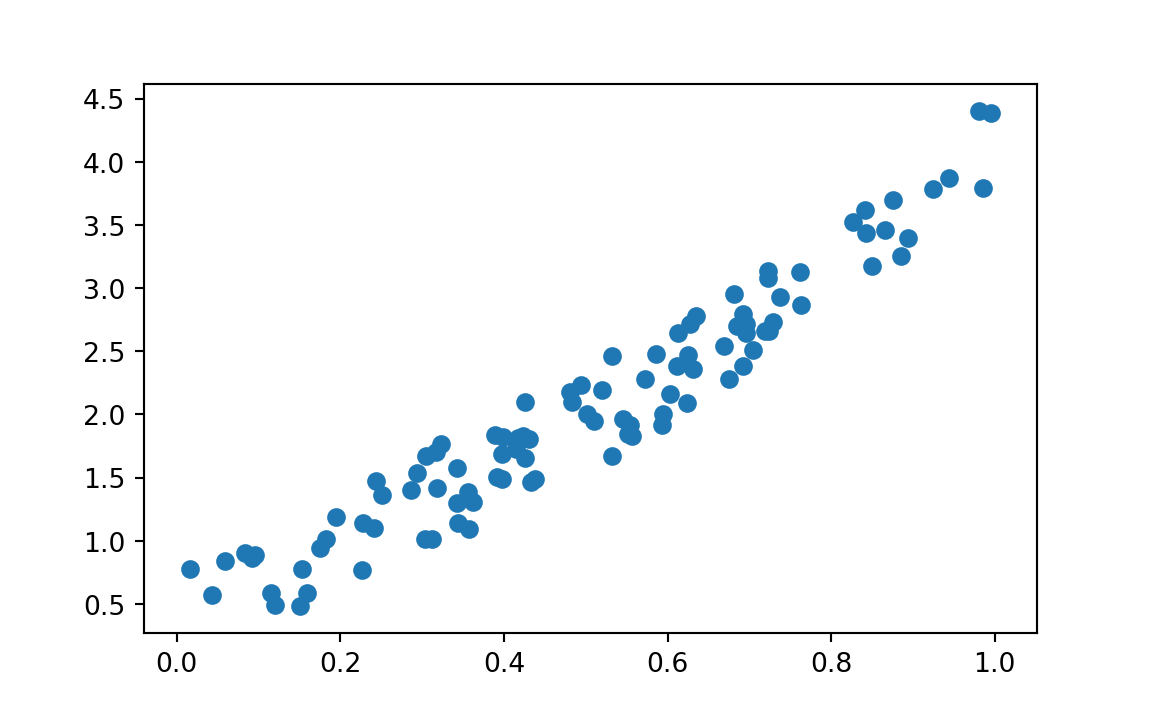
\includegraphics[width=0.7\linewidth]{0801-simple_regression_files/figure-latex/py-datasets-1}

This is the code in R:

\begin{Shaded}
\begin{Highlighting}[]
\NormalTok{np    <-}\StringTok{ }\KeywordTok{import}\NormalTok{(}\StringTok{"numpy"}\NormalTok{)}

\NormalTok{np}\OperatorTok{$}\NormalTok{random}\OperatorTok{$}\KeywordTok{seed}\NormalTok{(123L)}

\NormalTok{x =}\StringTok{ }\NormalTok{np}\OperatorTok{$}\NormalTok{random}\OperatorTok{$}\KeywordTok{rand}\NormalTok{(100L)}
\NormalTok{y =}\StringTok{ }\NormalTok{np}\OperatorTok{$}\KeywordTok{sin}\NormalTok{(x) }\OperatorTok{*}\StringTok{ }\NormalTok{np}\OperatorTok{$}\KeywordTok{power}\NormalTok{(x, 3L) }\OperatorTok{+}\StringTok{ }\DecValTok{3}\OperatorTok{*}\NormalTok{x }\OperatorTok{+}\StringTok{ }\NormalTok{np}\OperatorTok{$}\NormalTok{random}\OperatorTok{$}\KeywordTok{rand}\NormalTok{(100L)}\OperatorTok{*}\FloatTok{0.8}

\KeywordTok{plot}\NormalTok{(x, y)}
\end{Highlighting}
\end{Shaded}

\begin{center}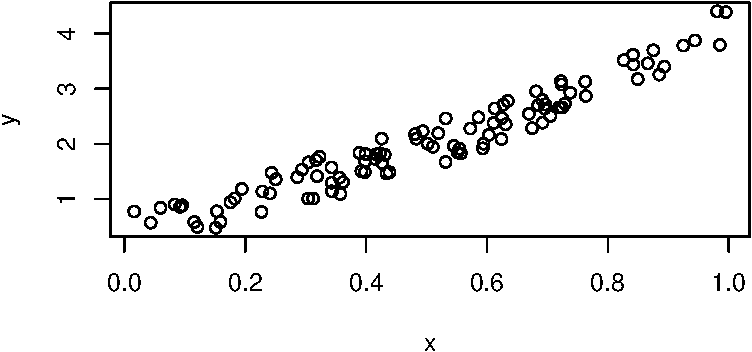
\includegraphics[width=0.7\linewidth]{0801-simple_regression_files/figure-latex/r-datasets-1} \end{center}

Before you start the training process, you need to convert the numpy array to Variables that supported by Torch and autograd.

\begin{Shaded}
\begin{Highlighting}[]
\CommentTok{# convert numpy array to tensor in shape of input size}
\NormalTok{x }\OperatorTok{=}\NormalTok{ torch.from_numpy(x.reshape(}\OperatorTok{-}\DecValTok{1}\NormalTok{,}\DecValTok{1}\NormalTok{)).}\BuiltInTok{float}\NormalTok{()}
\NormalTok{y }\OperatorTok{=}\NormalTok{ torch.from_numpy(y.reshape(}\OperatorTok{-}\DecValTok{1}\NormalTok{,}\DecValTok{1}\NormalTok{)).}\BuiltInTok{float}\NormalTok{()}
\BuiltInTok{print}\NormalTok{(x, y)}
\CommentTok{#> tensor([[0.6965],}
\CommentTok{#>         [0.2861],}
\CommentTok{#>         [0.2269],}
\CommentTok{#>         [0.5513],}
\CommentTok{#>         [0.7195],}
\CommentTok{#>         [0.4231],}
\CommentTok{#>         [0.9808],}
\CommentTok{#>         [0.6848],}
\CommentTok{#>         [0.4809],}
\CommentTok{#>         [0.3921],}
\CommentTok{#>         [0.3432],}
\CommentTok{#>         [0.7290],}
\CommentTok{#>         [0.4386],}
\CommentTok{#>         [0.0597],}
\CommentTok{#>         [0.3980],}
\CommentTok{#>         [0.7380],}
\CommentTok{#>         [0.1825],}
\CommentTok{#>         [0.1755],}
\CommentTok{#>         [0.5316],}
\CommentTok{#>         [0.5318],}
\CommentTok{#>         [0.6344],}
\CommentTok{#>         [0.8494],}
\CommentTok{#>         [0.7245],}
\CommentTok{#>         [0.6110],}
\CommentTok{#>         [0.7224],}
\CommentTok{#>         [0.3230],}
\CommentTok{#>         [0.3618],}
\CommentTok{#>         [0.2283],}
\CommentTok{#>         [0.2937],}
\CommentTok{#>         [0.6310],}
\CommentTok{#>         [0.0921],}
\CommentTok{#>         [0.4337],}
\CommentTok{#>         [0.4309],}
\CommentTok{#>         [0.4937],}
\CommentTok{#>         [0.4258],}
\CommentTok{#>         [0.3123],}
\CommentTok{#>         [0.4264],}
\CommentTok{#>         [0.8934],}
\CommentTok{#>         [0.9442],}
\CommentTok{#>         [0.5018],}
\CommentTok{#>         [0.6240],}
\CommentTok{#>         [0.1156],}
\CommentTok{#>         [0.3173],}
\CommentTok{#>         [0.4148],}
\CommentTok{#>         [0.8663],}
\CommentTok{#>         [0.2505],}
\CommentTok{#>         [0.4830],}
\CommentTok{#>         [0.9856],}
\CommentTok{#>         [0.5195],}
\CommentTok{#>         [0.6129],}
\CommentTok{#>         [0.1206],}
\CommentTok{#>         [0.8263],}
\CommentTok{#>         [0.6031],}
\CommentTok{#>         [0.5451],}
\CommentTok{#>         [0.3428],}
\CommentTok{#>         [0.3041],}
\CommentTok{#>         [0.4170],}
\CommentTok{#>         [0.6813],}
\CommentTok{#>         [0.8755],}
\CommentTok{#>         [0.5104],}
\CommentTok{#>         [0.6693],}
\CommentTok{#>         [0.5859],}
\CommentTok{#>         [0.6249],}
\CommentTok{#>         [0.6747],}
\CommentTok{#>         [0.8423],}
\CommentTok{#>         [0.0832],}
\CommentTok{#>         [0.7637],}
\CommentTok{#>         [0.2437],}
\CommentTok{#>         [0.1942],}
\CommentTok{#>         [0.5725],}
\CommentTok{#>         [0.0957],}
\CommentTok{#>         [0.8853],}
\CommentTok{#>         [0.6272],}
\CommentTok{#>         [0.7234],}
\CommentTok{#>         [0.0161],}
\CommentTok{#>         [0.5944],}
\CommentTok{#>         [0.5568],}
\CommentTok{#>         [0.1590],}
\CommentTok{#>         [0.1531],}
\CommentTok{#>         [0.6955],}
\CommentTok{#>         [0.3188],}
\CommentTok{#>         [0.6920],}
\CommentTok{#>         [0.5544],}
\CommentTok{#>         [0.3890],}
\CommentTok{#>         [0.9251],}
\CommentTok{#>         [0.8417],}
\CommentTok{#>         [0.3574],}
\CommentTok{#>         [0.0436],}
\CommentTok{#>         [0.3048],}
\CommentTok{#>         [0.3982],}
\CommentTok{#>         [0.7050],}
\CommentTok{#>         [0.9954],}
\CommentTok{#>         [0.3559],}
\CommentTok{#>         [0.7625],}
\CommentTok{#>         [0.5932],}
\CommentTok{#>         [0.6917],}
\CommentTok{#>         [0.1511],}
\CommentTok{#>         [0.3989],}
\CommentTok{#>         [0.2409],}
\CommentTok{#>         [0.3435]]) tensor([[2.7166],}
\CommentTok{#>         [1.3983],}
\CommentTok{#>         [0.7679],}
\CommentTok{#>         [1.8464],}
\CommentTok{#>         [2.6614],}
\CommentTok{#>         [1.8297],}
\CommentTok{#>         [4.4034],}
\CommentTok{#>         [2.7003],}
\CommentTok{#>         [2.1778],}
\CommentTok{#>         [1.5073],}
\CommentTok{#>         [1.2966],}
\CommentTok{#>         [2.7287],}
\CommentTok{#>         [1.4884],}
\CommentTok{#>         [0.8423],}
\CommentTok{#>         [1.4895],}
\CommentTok{#>         [2.9263],}
\CommentTok{#>         [1.0114],}
\CommentTok{#>         [0.9445],}
\CommentTok{#>         [1.6729],}
\CommentTok{#>         [2.4624],}
\CommentTok{#>         [2.7788],}
\CommentTok{#>         [3.1746],}
\CommentTok{#>         [2.6593],}
\CommentTok{#>         [2.3800],}
\CommentTok{#>         [3.1382],}
\CommentTok{#>         [1.7665],}
\CommentTok{#>         [1.3082],}
\CommentTok{#>         [1.1390],}
\CommentTok{#>         [1.5341],}
\CommentTok{#>         [2.3566],}
\CommentTok{#>         [0.8612],}
\CommentTok{#>         [1.4642],}
\CommentTok{#>         [1.8066],}
\CommentTok{#>         [2.2308],}
\CommentTok{#>         [2.0962],}
\CommentTok{#>         [1.0096],}
\CommentTok{#>         [1.6538],}
\CommentTok{#>         [3.3994],}
\CommentTok{#>         [3.8747],}
\CommentTok{#>         [2.0045],}
\CommentTok{#>         [2.0884],}
\CommentTok{#>         [0.5845],}
\CommentTok{#>         [1.7039],}
\CommentTok{#>         [1.7285],}
\CommentTok{#>         [3.4602],}
\CommentTok{#>         [1.3581],}
\CommentTok{#>         [2.0949],}
\CommentTok{#>         [3.7935],}
\CommentTok{#>         [2.1950],}
\CommentTok{#>         [2.6425],}
\CommentTok{#>         [0.4948],}
\CommentTok{#>         [3.5188],}
\CommentTok{#>         [2.1628],}
\CommentTok{#>         [1.9643],}
\CommentTok{#>         [1.5740],}
\CommentTok{#>         [1.0099],}
\CommentTok{#>         [1.8123],}
\CommentTok{#>         [2.9534],}
\CommentTok{#>         [3.6986],}
\CommentTok{#>         [1.9485],}
\CommentTok{#>         [2.5445],}
\CommentTok{#>         [2.4811],}
\CommentTok{#>         [2.4700],}
\CommentTok{#>         [2.2838],}
\CommentTok{#>         [3.4392],}
\CommentTok{#>         [0.9015],}
\CommentTok{#>         [2.8687],}
\CommentTok{#>         [1.4766],}
\CommentTok{#>         [1.1847],}
\CommentTok{#>         [2.2782],}
\CommentTok{#>         [0.8885],}
\CommentTok{#>         [3.2565],}
\CommentTok{#>         [2.7141],}
\CommentTok{#>         [3.0781],}
\CommentTok{#>         [0.7763],}
\CommentTok{#>         [2.0038],}
\CommentTok{#>         [1.8270],}
\CommentTok{#>         [0.5882],}
\CommentTok{#>         [0.7793],}
\CommentTok{#>         [2.6416],}
\CommentTok{#>         [1.4162],}
\CommentTok{#>         [2.3851],}
\CommentTok{#>         [1.9140],}
\CommentTok{#>         [1.8385],}
\CommentTok{#>         [3.7822],}
\CommentTok{#>         [3.6160],}
\CommentTok{#>         [1.0941],}
\CommentTok{#>         [0.5721],}
\CommentTok{#>         [1.6683],}
\CommentTok{#>         [1.6848],}
\CommentTok{#>         [2.5068],}
\CommentTok{#>         [4.3876],}
\CommentTok{#>         [1.3866],}
\CommentTok{#>         [3.1286],}
\CommentTok{#>         [1.9197],}
\CommentTok{#>         [2.7949],}
\CommentTok{#>         [0.4797],}
\CommentTok{#>         [1.8171],}
\CommentTok{#>         [1.1042],}
\CommentTok{#>         [1.1414]])}
\end{Highlighting}
\end{Shaded}

\hypertarget{code-in-r-1}{%
\subsection{Code in R}\label{code-in-r-1}}

Notice that before converting to a Torch tensor, we need first to convert the R numeric vector to a \texttt{numpy} array:

\begin{Shaded}
\begin{Highlighting}[]
\CommentTok{# convert numpy array to tensor in shape of input size}
\NormalTok{x <-}\StringTok{ }\KeywordTok{r_to_py}\NormalTok{(x)}
\NormalTok{y <-}\StringTok{ }\KeywordTok{r_to_py}\NormalTok{(y)}
\NormalTok{x =}\StringTok{ }\NormalTok{torch}\OperatorTok{$}\KeywordTok{from_numpy}\NormalTok{(x}\OperatorTok{$}\KeywordTok{reshape}\NormalTok{(}\OperatorTok{-}\NormalTok{1L, 1L)) }\CommentTok{#$float()}
\NormalTok{y =}\StringTok{ }\NormalTok{torch}\OperatorTok{$}\KeywordTok{from_numpy}\NormalTok{(y}\OperatorTok{$}\KeywordTok{reshape}\NormalTok{(}\OperatorTok{-}\NormalTok{1L, 1L)) }\CommentTok{#$float()}
\KeywordTok{print}\NormalTok{(x, y)}
\CommentTok{#> tensor([[0.6965],}
\CommentTok{#>         [0.2861],}
\CommentTok{#>         [0.2269],}
\CommentTok{#>         [0.5513],}
\CommentTok{#>         [0.7195],}
\CommentTok{#>         [0.4231],}
\CommentTok{#>         [0.9808],}
\CommentTok{#>         [0.6848],}
\CommentTok{#>         [0.4809],}
\CommentTok{#>         [0.3921],}
\CommentTok{#>         [0.3432],}
\CommentTok{#>         [0.7290],}
\CommentTok{#>         [0.4386],}
\CommentTok{#>         [0.0597],}
\CommentTok{#>         [0.3980],}
\CommentTok{#>         [0.7380],}
\CommentTok{#>         [0.1825],}
\CommentTok{#>         [0.1755],}
\CommentTok{#>         [0.5316],}
\CommentTok{#>         [0.5318],}
\CommentTok{#>         [0.6344],}
\CommentTok{#>         [0.8494],}
\CommentTok{#>         [0.7245],}
\CommentTok{#>         [0.6110],}
\CommentTok{#>         [0.7224],}
\CommentTok{#>         [0.3230],}
\CommentTok{#>         [0.3618],}
\CommentTok{#>         [0.2283],}
\CommentTok{#>         [0.2937],}
\CommentTok{#>         [0.6310],}
\CommentTok{#>         [0.0921],}
\CommentTok{#>         [0.4337],}
\CommentTok{#>         [0.4309],}
\CommentTok{#>         [0.4937],}
\CommentTok{#>         [0.4258],}
\CommentTok{#>         [0.3123],}
\CommentTok{#>         [0.4264],}
\CommentTok{#>         [0.8934],}
\CommentTok{#>         [0.9442],}
\CommentTok{#>         [0.5018],}
\CommentTok{#>         [0.6240],}
\CommentTok{#>         [0.1156],}
\CommentTok{#>         [0.3173],}
\CommentTok{#>         [0.4148],}
\CommentTok{#>         [0.8663],}
\CommentTok{#>         [0.2505],}
\CommentTok{#>         [0.4830],}
\CommentTok{#>         [0.9856],}
\CommentTok{#>         [0.5195],}
\CommentTok{#>         [0.6129],}
\CommentTok{#>         [0.1206],}
\CommentTok{#>         [0.8263],}
\CommentTok{#>         [0.6031],}
\CommentTok{#>         [0.5451],}
\CommentTok{#>         [0.3428],}
\CommentTok{#>         [0.3041],}
\CommentTok{#>         [0.4170],}
\CommentTok{#>         [0.6813],}
\CommentTok{#>         [0.8755],}
\CommentTok{#>         [0.5104],}
\CommentTok{#>         [0.6693],}
\CommentTok{#>         [0.5859],}
\CommentTok{#>         [0.6249],}
\CommentTok{#>         [0.6747],}
\CommentTok{#>         [0.8423],}
\CommentTok{#>         [0.0832],}
\CommentTok{#>         [0.7637],}
\CommentTok{#>         [0.2437],}
\CommentTok{#>         [0.1942],}
\CommentTok{#>         [0.5725],}
\CommentTok{#>         [0.0957],}
\CommentTok{#>         [0.8853],}
\CommentTok{#>         [0.6272],}
\CommentTok{#>         [0.7234],}
\CommentTok{#>         [0.0161],}
\CommentTok{#>         [0.5944],}
\CommentTok{#>         [0.5568],}
\CommentTok{#>         [0.1590],}
\CommentTok{#>         [0.1531],}
\CommentTok{#>         [0.6955],}
\CommentTok{#>         [0.3188],}
\CommentTok{#>         [0.6920],}
\CommentTok{#>         [0.5544],}
\CommentTok{#>         [0.3890],}
\CommentTok{#>         [0.9251],}
\CommentTok{#>         [0.8417],}
\CommentTok{#>         [0.3574],}
\CommentTok{#>         [0.0436],}
\CommentTok{#>         [0.3048],}
\CommentTok{#>         [0.3982],}
\CommentTok{#>         [0.7050],}
\CommentTok{#>         [0.9954],}
\CommentTok{#>         [0.3559],}
\CommentTok{#>         [0.7625],}
\CommentTok{#>         [0.5932],}
\CommentTok{#>         [0.6917],}
\CommentTok{#>         [0.1511],}
\CommentTok{#>         [0.3989],}
\CommentTok{#>         [0.2409],}
\CommentTok{#>         [0.3435]], dtype=torch.float64)}
\end{Highlighting}
\end{Shaded}

\hypertarget{optimizer-and-loss}{%
\section{Optimizer and Loss}\label{optimizer-and-loss}}

Next, you should define the Optimizer and the Loss Function for our training process.

\begin{Shaded}
\begin{Highlighting}[]
\CommentTok{# Define Optimizer and Loss Function}
\NormalTok{optimizer }\OperatorTok{=}\NormalTok{ torch.optim.SGD(net.parameters(), lr}\OperatorTok{=}\FloatTok{0.2}\NormalTok{)}
\NormalTok{loss_func }\OperatorTok{=}\NormalTok{ torch.nn.MSELoss()}
\BuiltInTok{print}\NormalTok{(optimizer)}
\CommentTok{#> SGD (}
\CommentTok{#> Parameter Group 0}
\CommentTok{#>     dampening: 0}
\CommentTok{#>     lr: 0.2}
\CommentTok{#>     momentum: 0}
\CommentTok{#>     nesterov: False}
\CommentTok{#>     weight_decay: 0}
\CommentTok{#> )}
\BuiltInTok{print}\NormalTok{(loss_func)}
\CommentTok{#> MSELoss()}
\end{Highlighting}
\end{Shaded}

\hypertarget{equivalent-code-in-r}{%
\subsection{Equivalent code in R}\label{equivalent-code-in-r}}

\begin{Shaded}
\begin{Highlighting}[]
\CommentTok{# Define Optimizer and Loss Function}
\NormalTok{optimizer <-}\StringTok{ }\NormalTok{torch}\OperatorTok{$}\NormalTok{optim}\OperatorTok{$}\KeywordTok{SGD}\NormalTok{(net}\OperatorTok{$}\KeywordTok{parameters}\NormalTok{(), }\DataTypeTok{lr=}\FloatTok{0.2}\NormalTok{)}
\NormalTok{loss_func <-}\StringTok{ }\NormalTok{torch}\OperatorTok{$}\NormalTok{nn}\OperatorTok{$}\KeywordTok{MSELoss}\NormalTok{()}
\KeywordTok{print}\NormalTok{(optimizer)}
\CommentTok{#> SGD (}
\CommentTok{#> Parameter Group 0}
\CommentTok{#>     dampening: 0}
\CommentTok{#>     lr: 0.2}
\CommentTok{#>     momentum: 0}
\CommentTok{#>     nesterov: False}
\CommentTok{#>     weight_decay: 0}
\CommentTok{#> )}
\KeywordTok{print}\NormalTok{(loss_func)}
\CommentTok{#> MSELoss()}
\end{Highlighting}
\end{Shaded}

\hypertarget{training}{%
\section{Training}\label{training}}

\hypertarget{code-in-python}{%
\subsection{Code in Python}\label{code-in-python}}

Now let's start our training process. With an epoch of 250, you will iterate our data to find the best value for our hyperparameters.

\begin{Shaded}
\begin{Highlighting}[]
\NormalTok{inputs }\OperatorTok{=}\NormalTok{ Variable(x)}
\NormalTok{outputs }\OperatorTok{=}\NormalTok{ Variable(y)}
\ControlFlowTok{for}\NormalTok{ i }\KeywordTok{in} \BuiltInTok{range}\NormalTok{(}\DecValTok{250}\NormalTok{):}
\NormalTok{   prediction }\OperatorTok{=}\NormalTok{ net(inputs)}
\NormalTok{   loss }\OperatorTok{=}\NormalTok{ loss_func(prediction, outputs) }
\NormalTok{   optimizer.zero_grad()}
\NormalTok{   loss.backward()        }
\NormalTok{   optimizer.step()       }

   \ControlFlowTok{if}\NormalTok{ i }\OperatorTok{%} \DecValTok{10} \OperatorTok{==} \DecValTok{0}\NormalTok{:}
       \CommentTok{# plot and show learning process}
\NormalTok{       plt.cla()}
\NormalTok{       plt.scatter(x.data.numpy(), y.data.numpy())}
\NormalTok{       plt.plot(x.data.numpy(), prediction.data.numpy(), }\StringTok{'r-'}\NormalTok{, lw}\OperatorTok{=}\DecValTok{2}\NormalTok{)}
\NormalTok{       plt.text(}\FloatTok{0.5}\NormalTok{, }\DecValTok{0}\NormalTok{, }\StringTok{'Loss=}\SpecialCharTok\NormalTok{ loss.data.numpy(), fontdict}\OperatorTok{=}\NormalTok{\{}\StringTok{'size'}\NormalTok{: }\DecValTok{10}\NormalTok{, }\StringTok{'color'}\NormalTok{:  }\StringTok{'red'}\NormalTok{\})}
\NormalTok{       plt.pause(}\FloatTok{0.1}\NormalTok{)}
\end{Highlighting}
\end{Shaded}

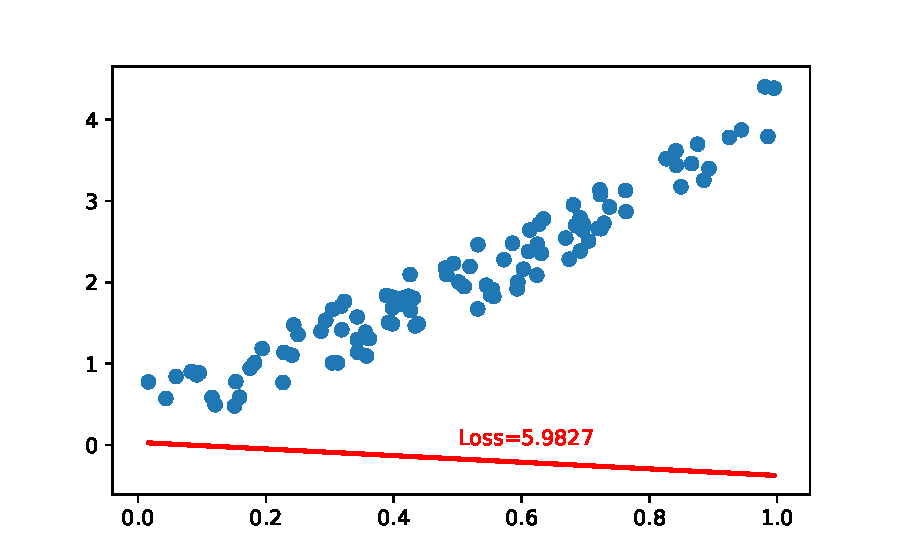
\includegraphics[width=0.7\linewidth]{0801-simple_regression_files/figure-latex/py-iterate-1} 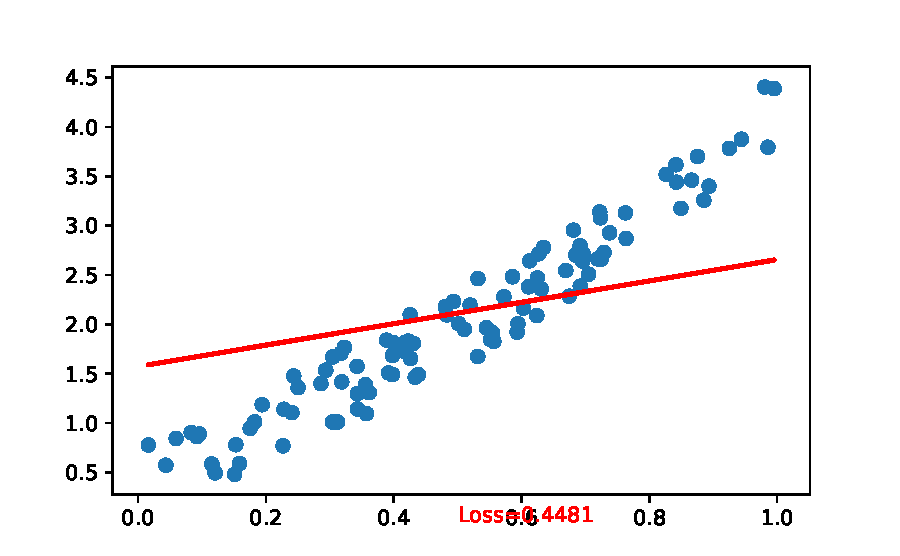
\includegraphics[width=0.7\linewidth]{0801-simple_regression_files/figure-latex/py-iterate-2} 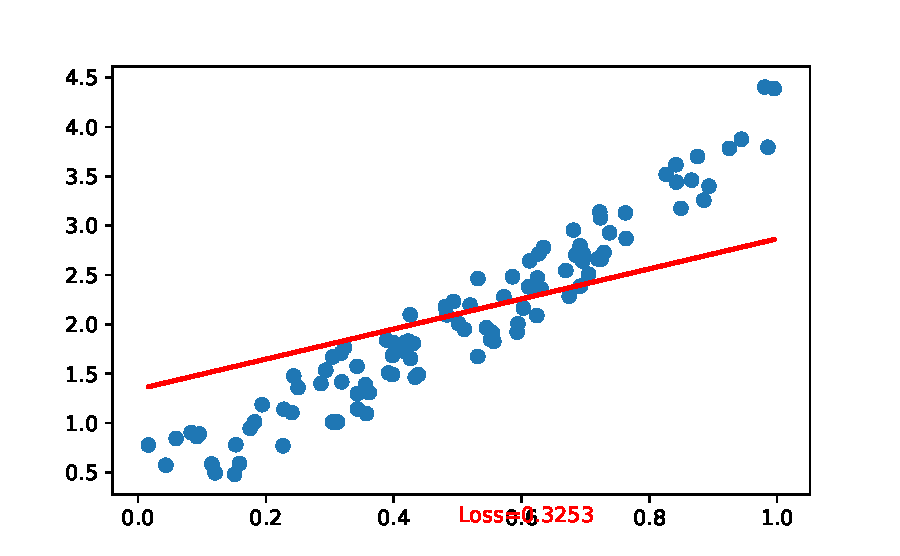
\includegraphics[width=0.7\linewidth]{0801-simple_regression_files/figure-latex/py-iterate-3} 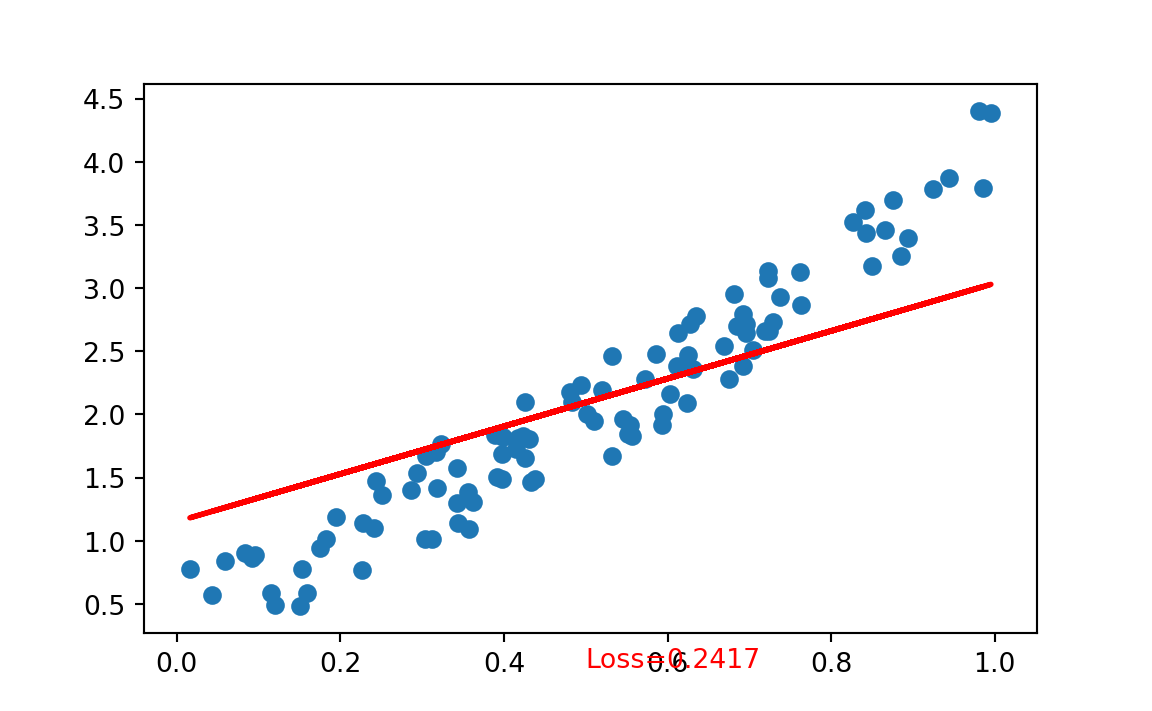
\includegraphics[width=0.7\linewidth]{0801-simple_regression_files/figure-latex/py-iterate-4} 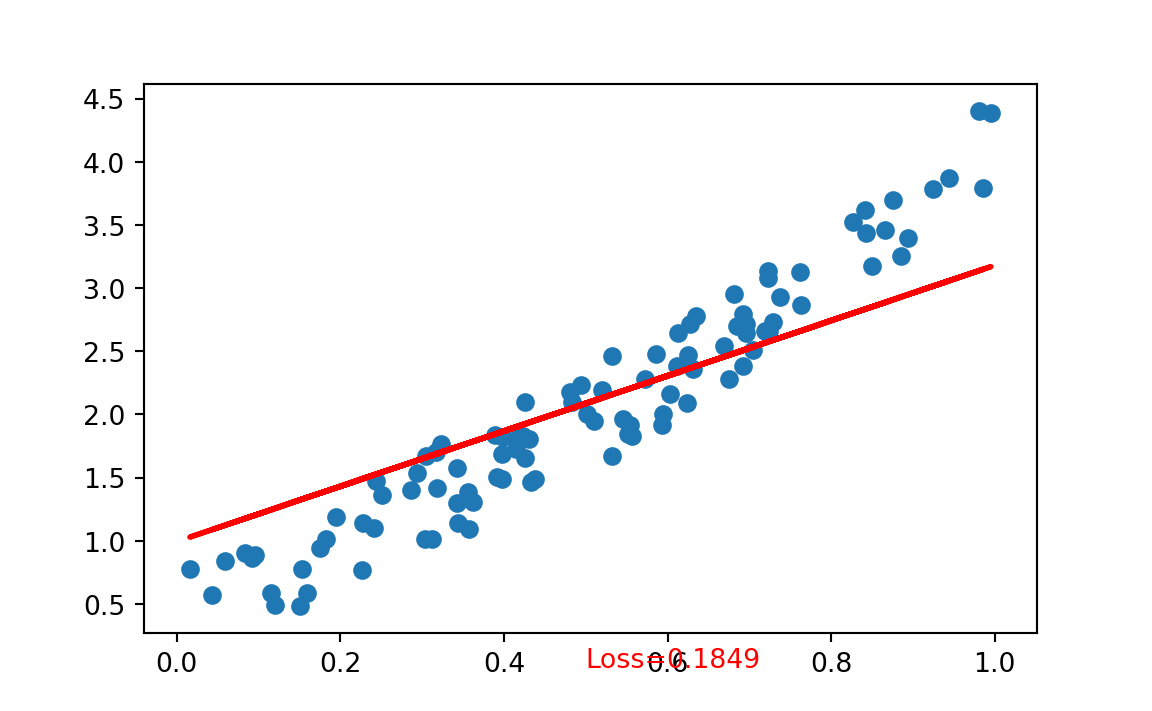
\includegraphics[width=0.7\linewidth]{0801-simple_regression_files/figure-latex/py-iterate-5} 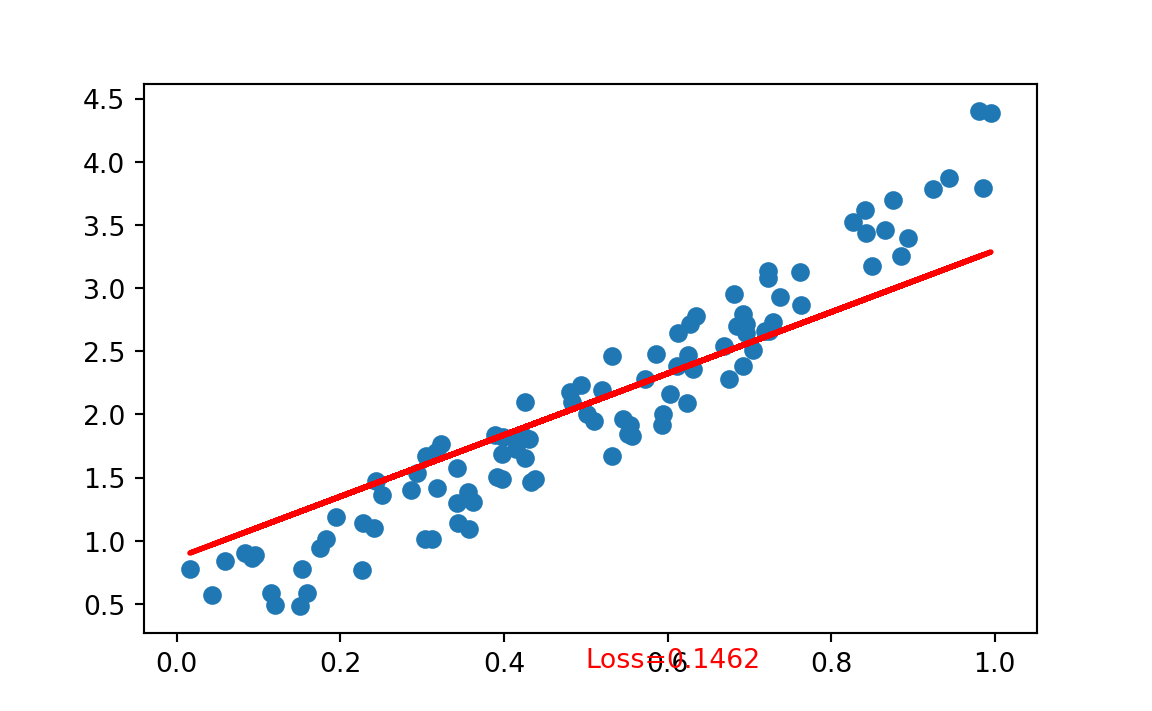
\includegraphics[width=0.7\linewidth]{0801-simple_regression_files/figure-latex/py-iterate-6} 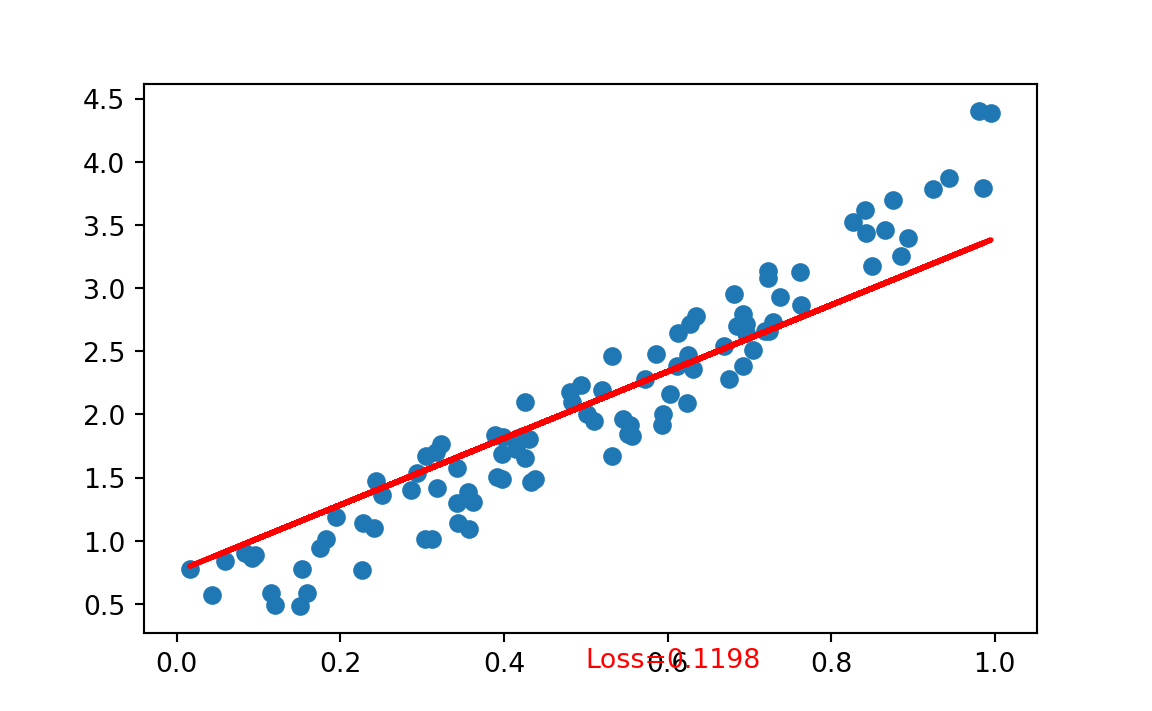
\includegraphics[width=0.7\linewidth]{0801-simple_regression_files/figure-latex/py-iterate-7} 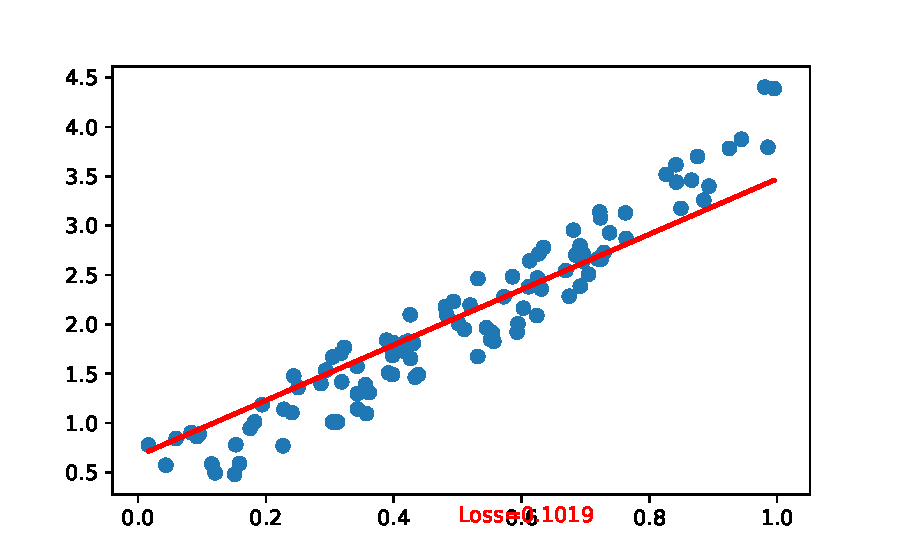
\includegraphics[width=0.7\linewidth]{0801-simple_regression_files/figure-latex/py-iterate-8} 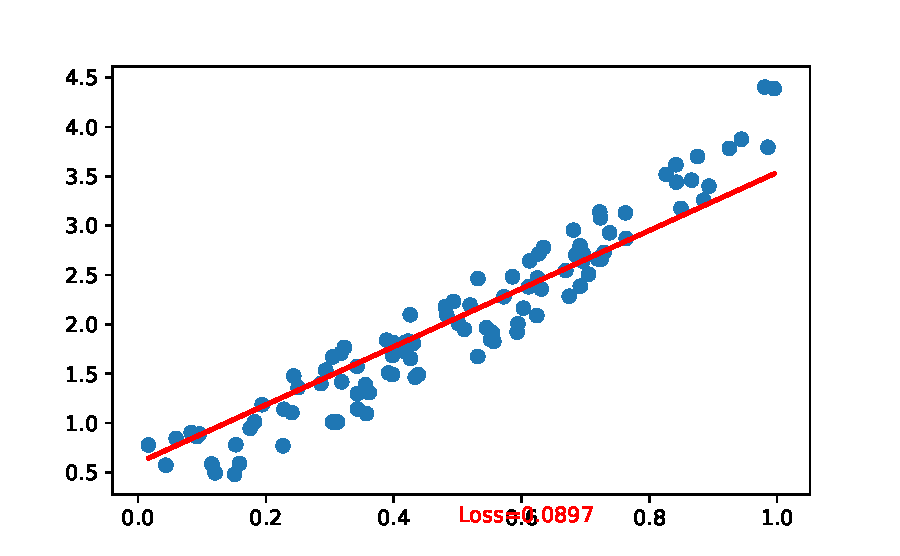
\includegraphics[width=0.7\linewidth]{0801-simple_regression_files/figure-latex/py-iterate-9} 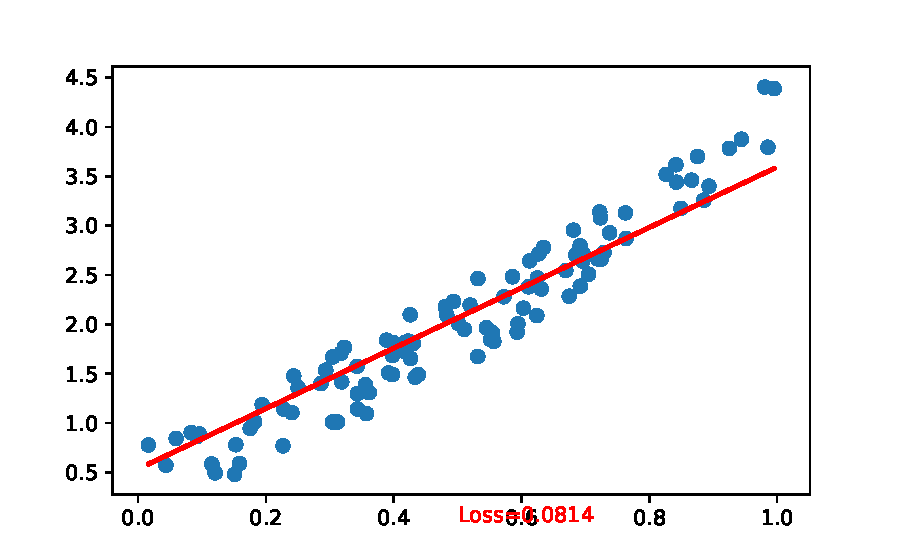
\includegraphics[width=0.7\linewidth]{0801-simple_regression_files/figure-latex/py-iterate-10} 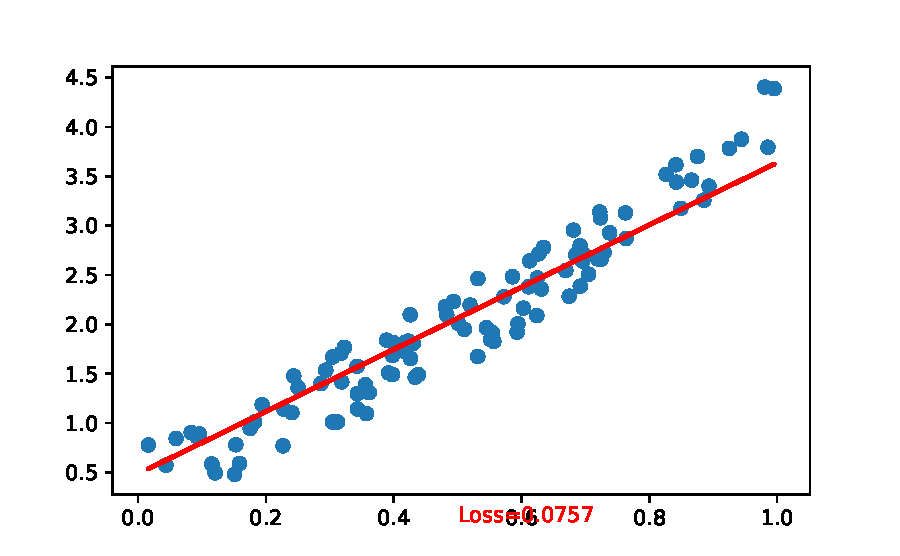
\includegraphics[width=0.7\linewidth]{0801-simple_regression_files/figure-latex/py-iterate-11} 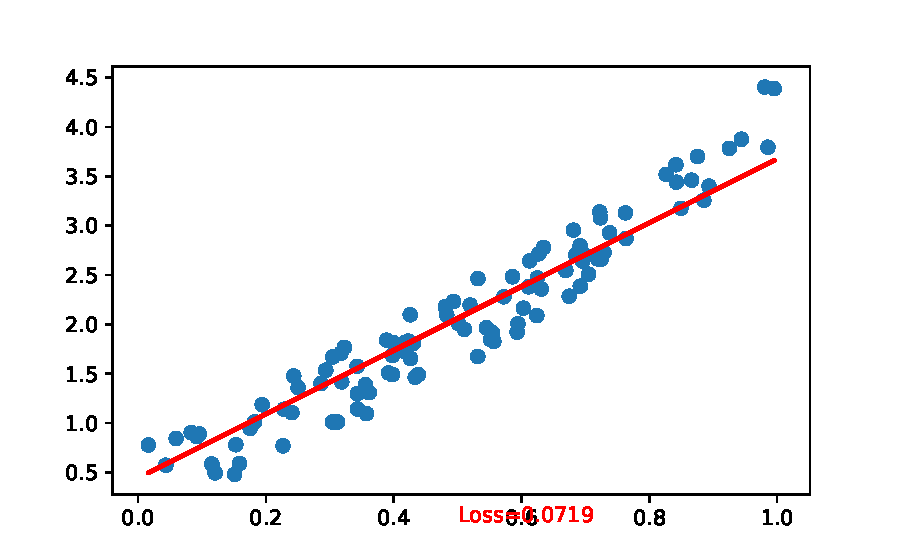
\includegraphics[width=0.7\linewidth]{0801-simple_regression_files/figure-latex/py-iterate-12} 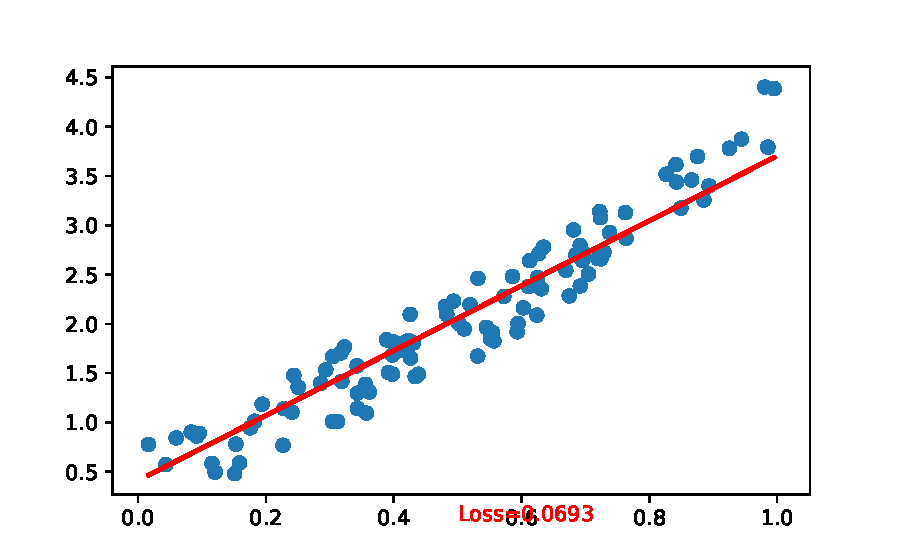
\includegraphics[width=0.7\linewidth]{0801-simple_regression_files/figure-latex/py-iterate-13} 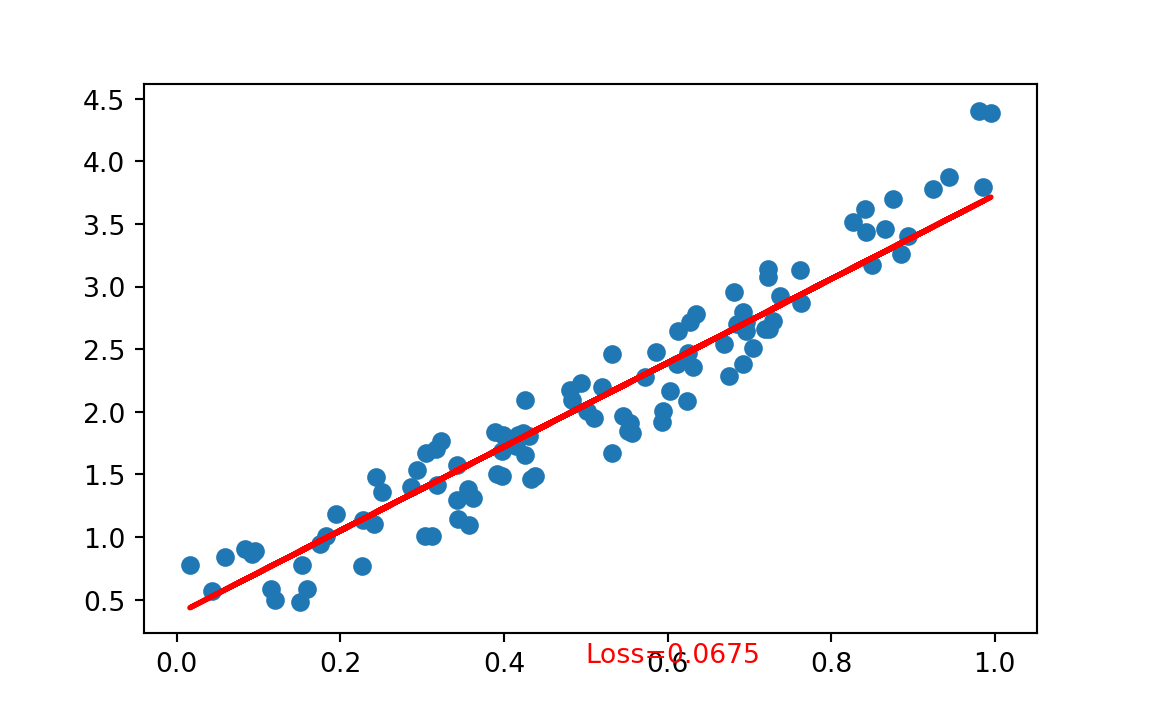
\includegraphics[width=0.7\linewidth]{0801-simple_regression_files/figure-latex/py-iterate-14} 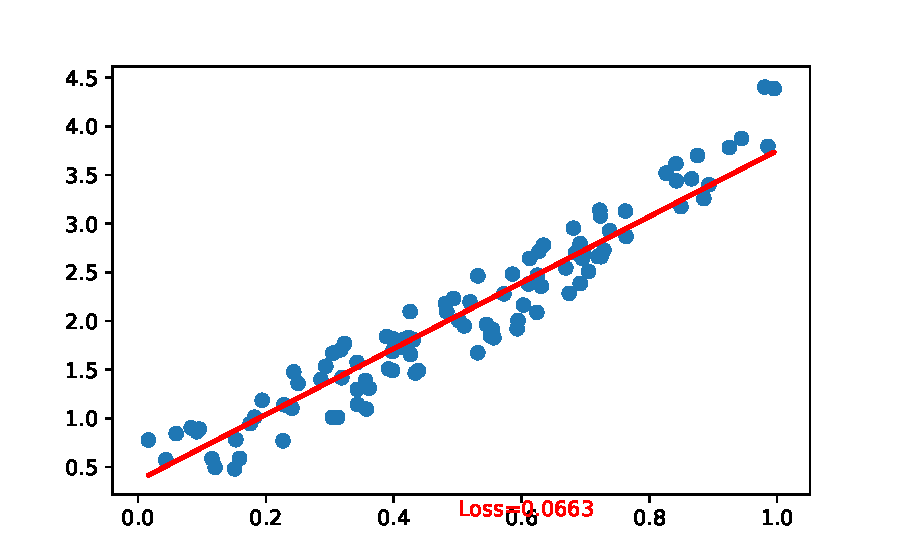
\includegraphics[width=0.7\linewidth]{0801-simple_regression_files/figure-latex/py-iterate-15} 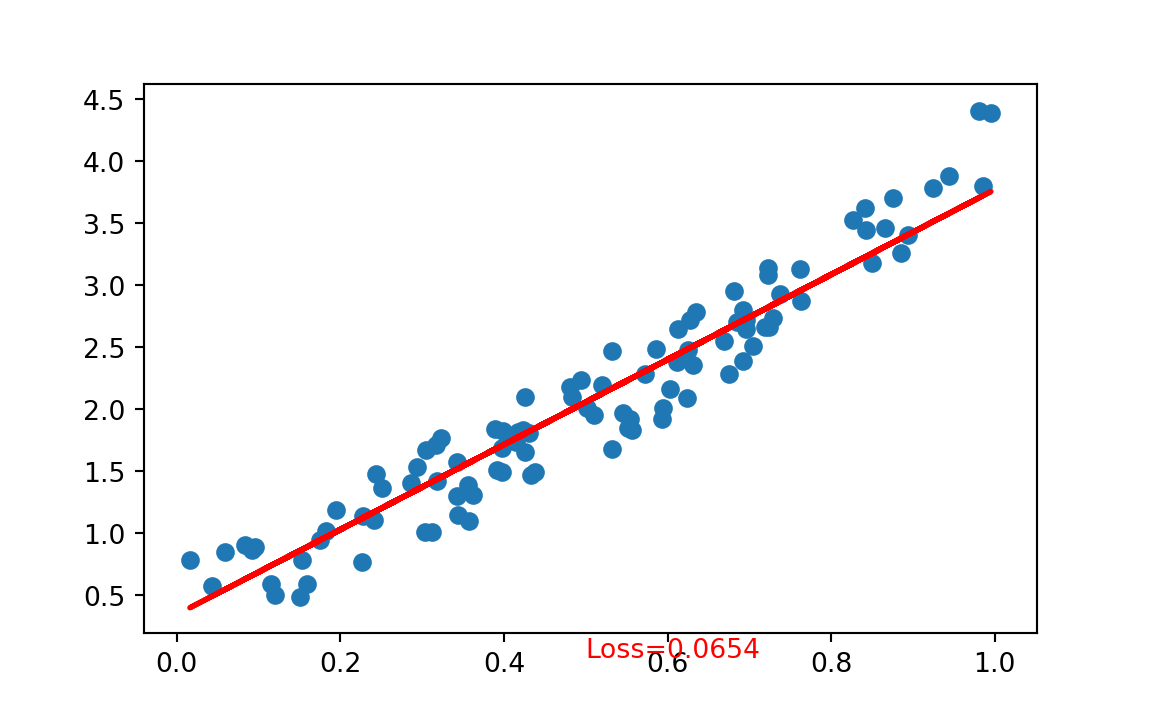
\includegraphics[width=0.7\linewidth]{0801-simple_regression_files/figure-latex/py-iterate-16} 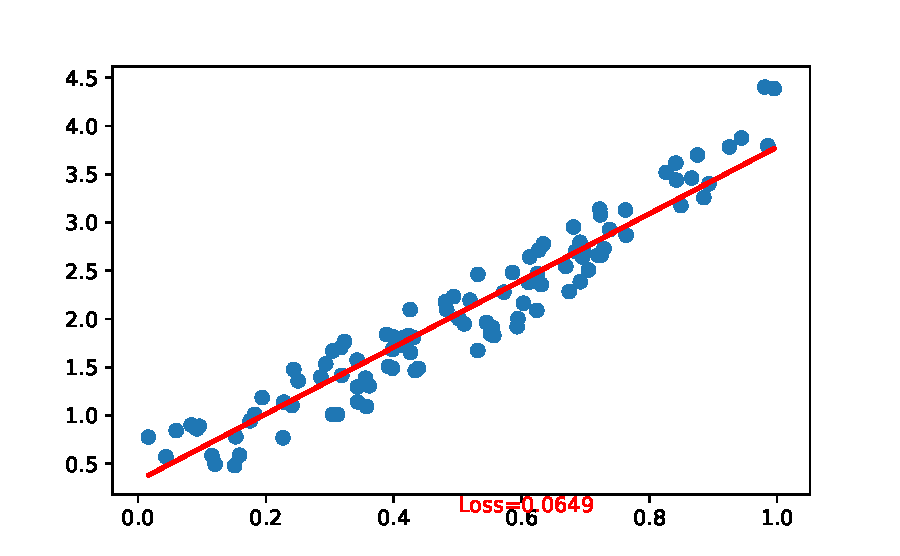
\includegraphics[width=0.7\linewidth]{0801-simple_regression_files/figure-latex/py-iterate-17} 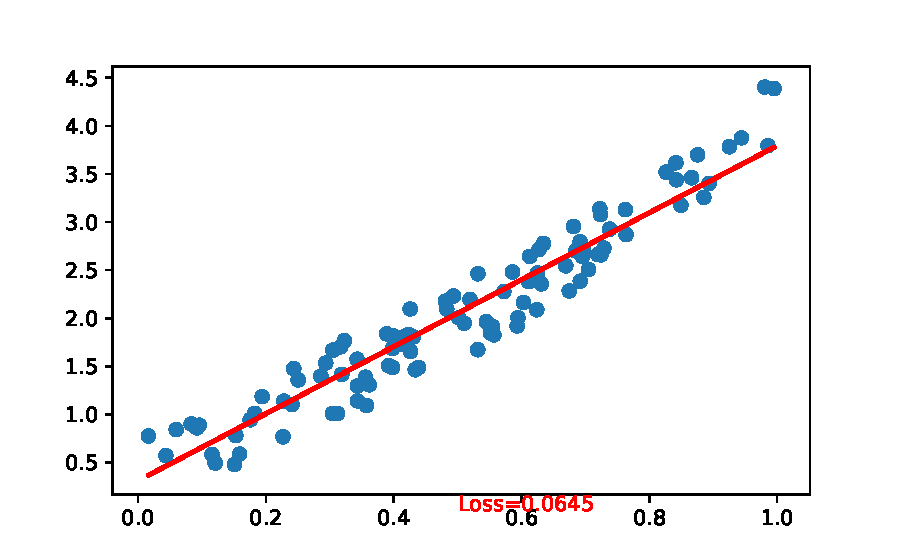
\includegraphics[width=0.7\linewidth]{0801-simple_regression_files/figure-latex/py-iterate-18} 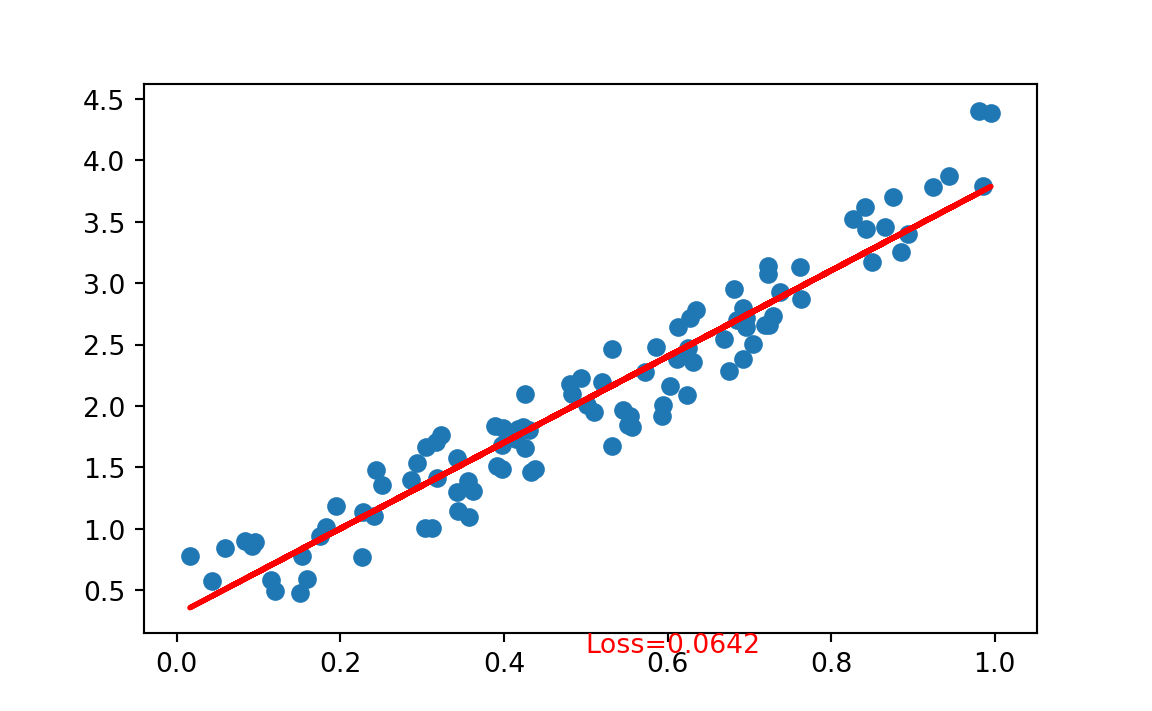
\includegraphics[width=0.7\linewidth]{0801-simple_regression_files/figure-latex/py-iterate-19} 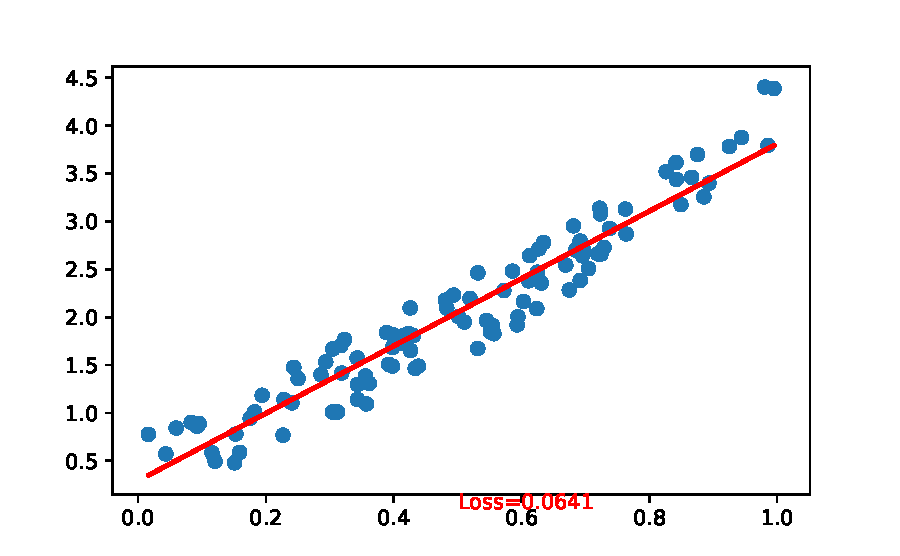
\includegraphics[width=0.7\linewidth]{0801-simple_regression_files/figure-latex/py-iterate-20} 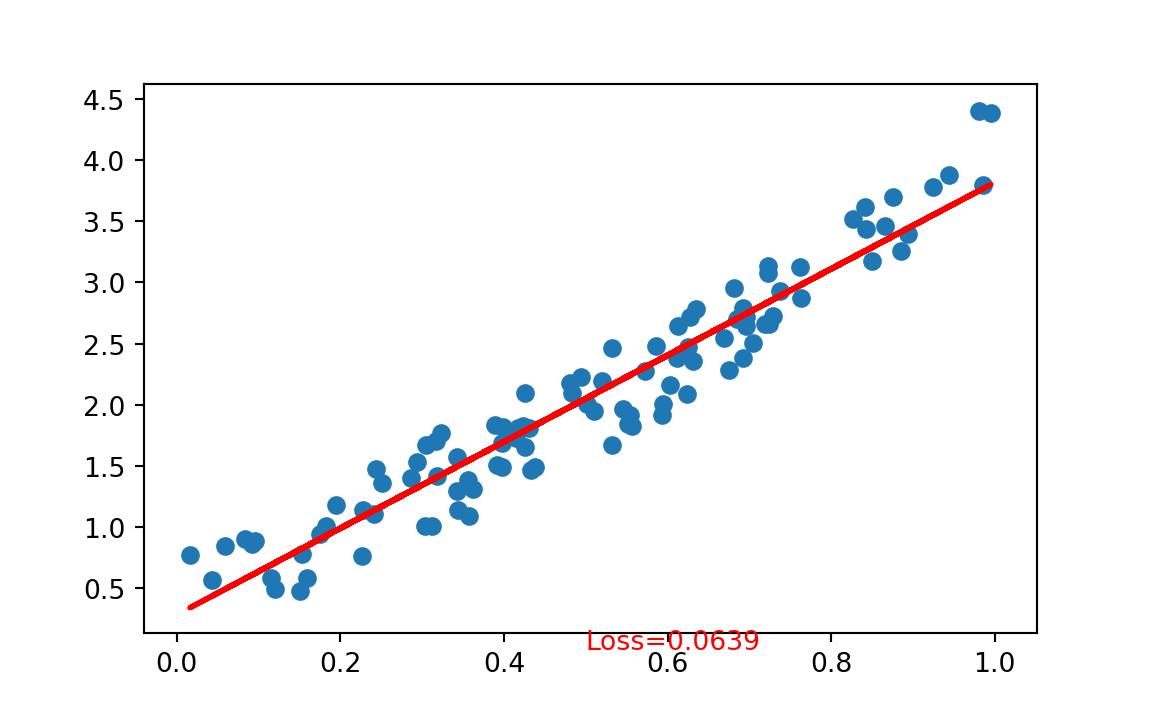
\includegraphics[width=0.7\linewidth]{0801-simple_regression_files/figure-latex/py-iterate-21} 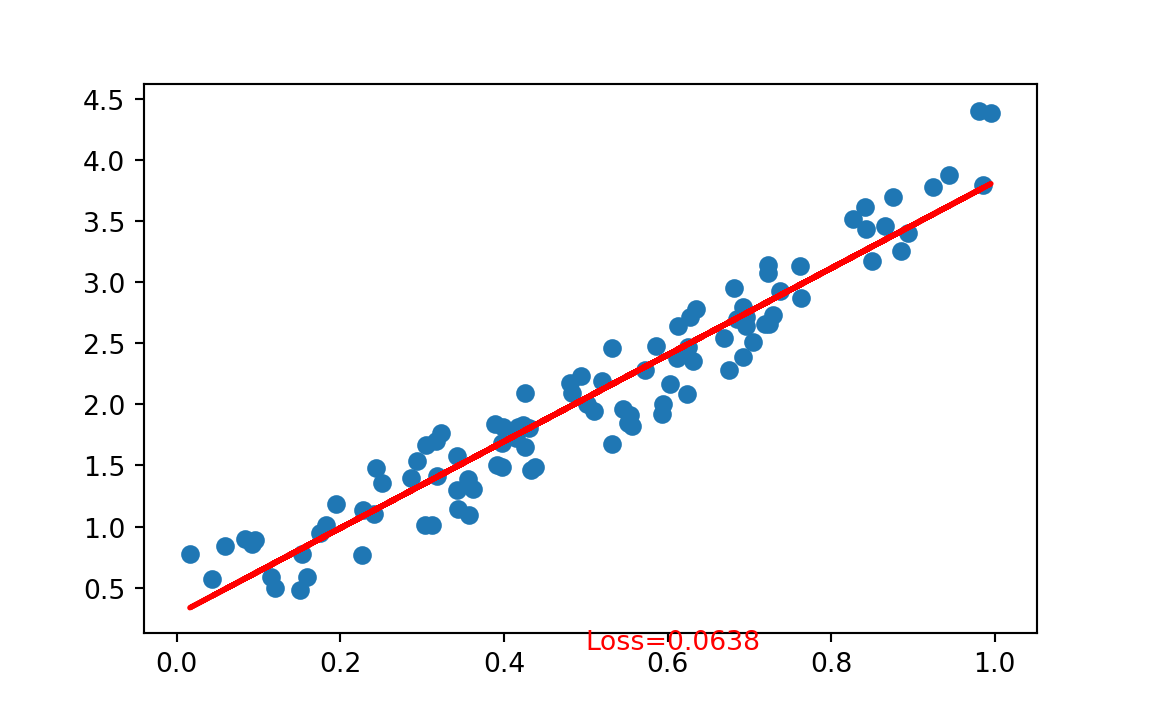
\includegraphics[width=0.7\linewidth]{0801-simple_regression_files/figure-latex/py-iterate-22} 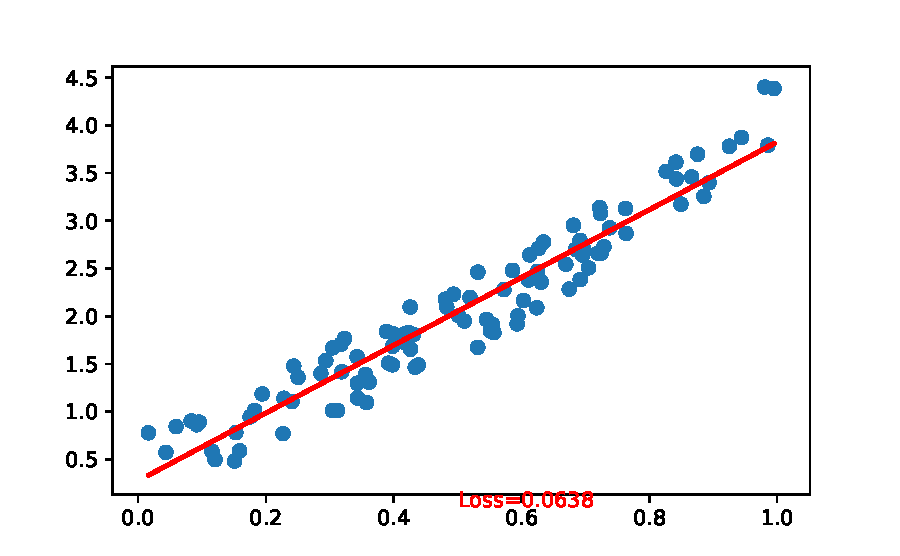
\includegraphics[width=0.7\linewidth]{0801-simple_regression_files/figure-latex/py-iterate-23} 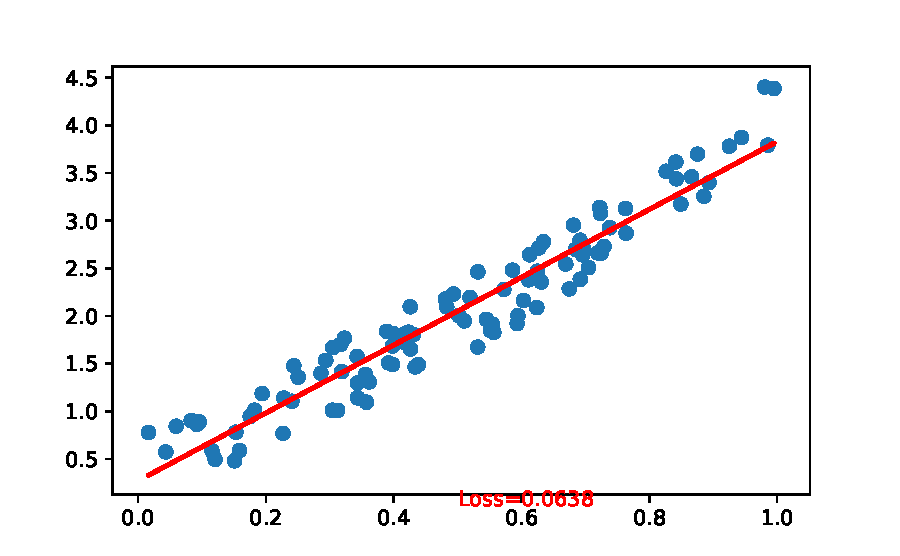
\includegraphics[width=0.7\linewidth]{0801-simple_regression_files/figure-latex/py-iterate-24} 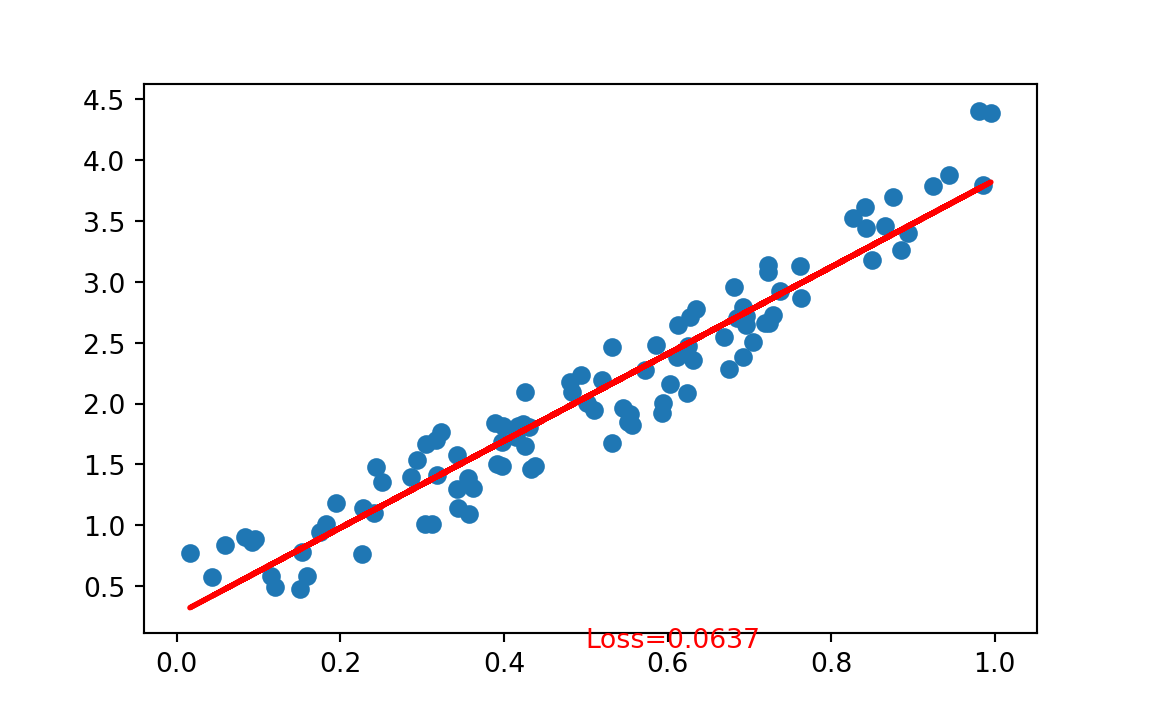
\includegraphics[width=0.7\linewidth]{0801-simple_regression_files/figure-latex/py-iterate-25}

\begin{Shaded}
\begin{Highlighting}[]
\NormalTok{plt.show()}
\end{Highlighting}
\end{Shaded}


\includegraphics[width=0.7\linewidth]{0801-simple_regression_files/figure-latex/py-iterate-26}

\hypertarget{code-in-r-2}{%
\subsection{Code in R}\label{code-in-r-2}}

\begin{Shaded}
\begin{Highlighting}[]
\NormalTok{x =}\StringTok{ }\NormalTok{x}\OperatorTok{$}\KeywordTok{type}\NormalTok{(torch}\OperatorTok{$}\NormalTok{FloatTensor)   }\CommentTok{# make it a a FloatTensor}
\NormalTok{y =}\StringTok{ }\NormalTok{y}\OperatorTok{$}\KeywordTok{type}\NormalTok{(torch}\OperatorTok{$}\NormalTok{FloatTensor)}

\NormalTok{inputs =}\StringTok{ }\KeywordTok{Variable}\NormalTok{(x)}
\NormalTok{outputs =}\StringTok{ }\KeywordTok{Variable}\NormalTok{(y)}
\KeywordTok{plot}\NormalTok{(x}\OperatorTok{$}\NormalTok{data}\OperatorTok{$}\KeywordTok{numpy}\NormalTok{(), y}\OperatorTok{$}\NormalTok{data}\OperatorTok{$}\KeywordTok{numpy}\NormalTok{(), }\DataTypeTok{col =} \StringTok{"blue"}\NormalTok{)}
\ControlFlowTok{for}\NormalTok{ (i }\ControlFlowTok{in} \DecValTok{1}\OperatorTok{:}\DecValTok{250}\NormalTok{) \{}
\NormalTok{   prediction =}\StringTok{ }\KeywordTok{net}\NormalTok{(inputs)}
\NormalTok{   loss =}\StringTok{ }\KeywordTok{loss_func}\NormalTok{(prediction, outputs)}
\NormalTok{   optimizer}\OperatorTok{$}\KeywordTok{zero_grad}\NormalTok{()}
\NormalTok{   loss}\OperatorTok{$}\KeywordTok{backward}\NormalTok{()}
\NormalTok{   optimizer}\OperatorTok{$}\KeywordTok{step}\NormalTok{()}

   \ControlFlowTok{if}\NormalTok{ (i }\OperatorTok\StringTok{ }\DecValTok{10} \OperatorTok{==}\StringTok{ }\DecValTok{0}\NormalTok{) \{}
       \CommentTok{# plot and show learning process}
      \CommentTok{# points(x$data$numpy(), y$data$numpy())}
      \KeywordTok{points}\NormalTok{(x}\OperatorTok{$}\NormalTok{data}\OperatorTok{$}\KeywordTok{numpy}\NormalTok{(), prediction}\OperatorTok{$}\NormalTok{data}\OperatorTok{$}\KeywordTok{numpy}\NormalTok{(), }\DataTypeTok{col=}\StringTok{"red"}\NormalTok{)}
       \CommentTok{# cat(i, loss$data$numpy(), "\textbackslash{}n")}
\NormalTok{   \}}
\NormalTok{\}}
\end{Highlighting}
\end{Shaded}

\begin{center}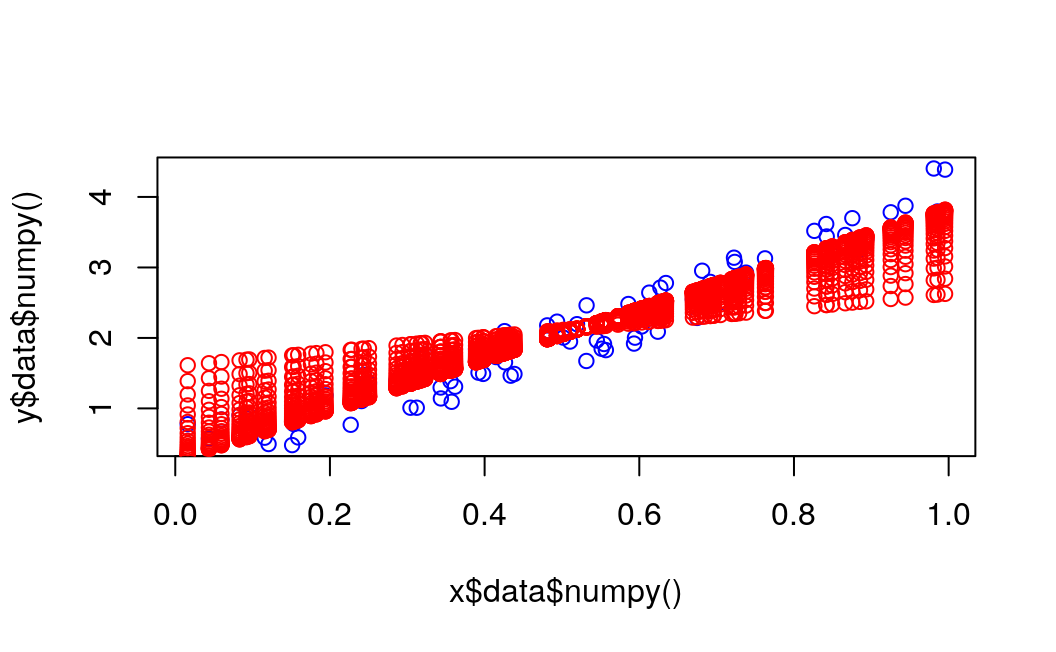
\includegraphics[width=0.7\linewidth]{0801-simple_regression_files/figure-latex/r-iterate-1} \end{center}

\hypertarget{result}{%
\section{Result}\label{result}}

As you can see below, you successfully performed regression with a neural network. Actually, on every iteration, the red line in the plot will update and change its position to fit the data. But in this picture, you only show you the final result

\hypertarget{autograd}{%
\chapter{Autograd}\label{autograd}}

Source: \url{https://github.com/jcjohnson/pytorch-examples\#pytorch-autograd}

\begin{Shaded}
\begin{Highlighting}[]
\KeywordTok{library}\NormalTok{(rTorch)}
\end{Highlighting}
\end{Shaded}

\hypertarget{python-code}{%
\section{Python code}\label{python-code}}

\begin{Shaded}
\begin{Highlighting}[]
\CommentTok{# Do not print from a function. Similar functionality to R invisible()}
\CommentTok{# https://stackoverflow.com/a/45669280/5270873}
\ImportTok{import}\NormalTok{ os, sys}

\KeywordTok{class}\NormalTok{ HiddenPrints:}
    \KeywordTok{def} \FunctionTok{__enter__}\NormalTok{(}\VariableTok{self}\NormalTok{):}
        \VariableTok{self}\NormalTok{._original_stdout }\OperatorTok{=}\NormalTok{ sys.stdout}
\NormalTok{        sys.stdout }\OperatorTok{=} \BuiltInTok{open}\NormalTok{(os.devnull, }\StringTok{'w'}\NormalTok{)}

    \KeywordTok{def} \FunctionTok{__exit__}\NormalTok{(}\VariableTok{self}\NormalTok{, exc_type, exc_val, exc_tb):}
\NormalTok{        sys.stdout.close()}
\NormalTok{        sys.stdout }\OperatorTok{=} \VariableTok{self}\NormalTok{._original_stdout}
\end{Highlighting}
\end{Shaded}

\begin{Shaded}
\begin{Highlighting}[]
\CommentTok{# Code in file autograd/two_layer_net_autograd.py}
\ImportTok{import}\NormalTok{ torch}
\NormalTok{device }\OperatorTok{=}\NormalTok{ torch.device(}\StringTok{'cpu'}\NormalTok{)}
\CommentTok{# device = torch.device('cuda') # Uncomment this to run on GPU}

\NormalTok{torch.manual_seed(}\DecValTok{0}\NormalTok{)}

\CommentTok{# N is batch size; D_in is input dimension;}
\CommentTok{# H is hidden dimension; D_out is output dimension.}
\CommentTok{#> <torch._C.Generator object at 0x7f9444efdb90>}
\NormalTok{N, D_in, H, D_out }\OperatorTok{=} \DecValTok{64}\NormalTok{, }\DecValTok{1000}\NormalTok{, }\DecValTok{100}\NormalTok{, }\DecValTok{10}

\CommentTok{# Create random Tensors to hold input and outputs}
\NormalTok{x }\OperatorTok{=}\NormalTok{ torch.randn(N, D_in, device}\OperatorTok{=}\NormalTok{device)}
\NormalTok{y }\OperatorTok{=}\NormalTok{ torch.randn(N, D_out, device}\OperatorTok{=}\NormalTok{device)}

\CommentTok{# Create random Tensors for weights; setting requires_grad=True means that we}
\CommentTok{# want to compute gradients for these Tensors during the backward pass.}
\NormalTok{w1 }\OperatorTok{=}\NormalTok{ torch.randn(D_in, H, device}\OperatorTok{=}\NormalTok{device, requires_grad}\OperatorTok{=}\VariableTok{True}\NormalTok{)}
\NormalTok{w2 }\OperatorTok{=}\NormalTok{ torch.randn(H, D_out, device}\OperatorTok{=}\NormalTok{device, requires_grad}\OperatorTok{=}\VariableTok{True}\NormalTok{)}

\NormalTok{learning_rate }\OperatorTok{=} \FloatTok{1e-6}

\ControlFlowTok{for}\NormalTok{ t }\KeywordTok{in} \BuiltInTok{range}\NormalTok{(}\DecValTok{5}\NormalTok{):}
  \CommentTok{# Forward pass: compute predicted y using operations on Tensors. Since w1 and}
  \CommentTok{# w2 have requires_grad=True, operations involving these Tensors will cause}
  \CommentTok{# PyTorch to build a computational graph, allowing automatic computation of}
  \CommentTok{# gradients. Since we are no longer implementing the backward pass by hand we}
  \CommentTok{# don't need to keep references to intermediate values.}
\NormalTok{  y_pred }\OperatorTok{=}\NormalTok{ x.mm(w1).clamp(}\BuiltInTok{min}\OperatorTok{=}\DecValTok{0}\NormalTok{).mm(w2)}
  
  \CommentTok{# Compute and print loss. Loss is a Tensor of shape (), and loss.item()}
  \CommentTok{# is a Python number giving its value.}
\NormalTok{  loss }\OperatorTok{=}\NormalTok{ (y_pred }\OperatorTok{-}\NormalTok{ y).}\BuiltInTok{pow}\NormalTok{(}\DecValTok{2}\NormalTok{).}\BuiltInTok{sum}\NormalTok{()}
  \BuiltInTok{print}\NormalTok{(t, loss.item())}

  \CommentTok{# Use autograd to compute the backward pass. This call will compute the}
  \CommentTok{# gradient of loss with respect to all Tensors with requires_grad=True.}
  \CommentTok{# After this call w1.grad and w2.grad will be Tensors holding the gradient}
  \CommentTok{# of the loss with respect to w1 and w2 respectively.}
\NormalTok{  loss.backward()}

  \CommentTok{# Update weights using gradient descent. For this step we just want to mutate}
  \CommentTok{# the values of w1 and w2 in-place; we don't want to build up a computational}
  \CommentTok{# graph for the update steps, so we use the torch.no_grad() context manager}
  \CommentTok{# to prevent PyTorch from building a computational graph for the updates}
  \ControlFlowTok{with}\NormalTok{ torch.no_grad():}
\NormalTok{    w1 }\OperatorTok{-=}\NormalTok{ learning_rate }\OperatorTok{*}\NormalTok{ w1.grad}
\NormalTok{    w2 }\OperatorTok{-=}\NormalTok{ learning_rate }\OperatorTok{*}\NormalTok{ w2.grad}

    \CommentTok{# Manually zero the gradients after running the backward pass}
    \ControlFlowTok{with}\NormalTok{ HiddenPrints():   }\CommentTok{# this would be the equivalent of invisible() in R}
\NormalTok{      w1.grad.zero_()}
\NormalTok{      w2.grad.zero_()}
\CommentTok{#> 0 29428666.0}
\CommentTok{#> 1 22739450.0}
\CommentTok{#> 2 20605262.0}
\CommentTok{#> 3 19520376.0}
\CommentTok{#> 4 17810228.0}
\end{Highlighting}
\end{Shaded}

\hypertarget{r-code}{%
\section{R code}\label{r-code}}

\begin{Shaded}
\begin{Highlighting}[]
\CommentTok{# library(reticulate) # originally qwe used reticulate}
\KeywordTok{library}\NormalTok{(rTorch)}

\NormalTok{torch  =}\StringTok{ }\KeywordTok{import}\NormalTok{(}\StringTok{"torch"}\NormalTok{)}
\NormalTok{device =}\StringTok{ }\NormalTok{torch}\OperatorTok{$}\KeywordTok{device}\NormalTok{(}\StringTok{'cpu'}\NormalTok{)}
\CommentTok{# device = torch.device('cuda') # Uncomment this to run on GPU}

\NormalTok{torch}\OperatorTok{$}\KeywordTok{manual_seed}\NormalTok{(}\DecValTok{0}\NormalTok{)}
\CommentTok{#> <torch._C.Generator>}

\CommentTok{# N is batch size; D_in is input dimension;}
\CommentTok{# H is hidden dimension; D_out is output dimension.}
\NormalTok{N <-}\StringTok{ }\NormalTok{64L; D_in <-}\StringTok{ }\NormalTok{1000L; H <-}\StringTok{ }\NormalTok{100L; D_out <-}\StringTok{ }\NormalTok{10L}

\CommentTok{# Create random Tensors to hold inputs and outputs}
\NormalTok{x =}\StringTok{ }\NormalTok{torch}\OperatorTok{$}\KeywordTok{randn}\NormalTok{(N, D_in, }\DataTypeTok{device=}\NormalTok{device)}
\NormalTok{y =}\StringTok{ }\NormalTok{torch}\OperatorTok{$}\KeywordTok{randn}\NormalTok{(N, D_out, }\DataTypeTok{device=}\NormalTok{device)}

\CommentTok{# Create random Tensors for weights; setting requires_grad=True means that we}
\CommentTok{# want to compute gradients for these Tensors during the backward pass.}
\NormalTok{w1 =}\StringTok{ }\NormalTok{torch}\OperatorTok{$}\KeywordTok{randn}\NormalTok{(D_in, H, }\DataTypeTok{device=}\NormalTok{device, }\DataTypeTok{requires_grad=}\OtherTok{TRUE}\NormalTok{)}
\NormalTok{w2 =}\StringTok{ }\NormalTok{torch}\OperatorTok{$}\KeywordTok{randn}\NormalTok{(H, D_out, }\DataTypeTok{device=}\NormalTok{device, }\DataTypeTok{requires_grad=}\OtherTok{TRUE}\NormalTok{)}

\NormalTok{learning_rate =}\StringTok{ }\NormalTok{torch}\OperatorTok{$}\KeywordTok{scalar_tensor}\NormalTok{(}\FloatTok{1e-6}\NormalTok{)}

\ControlFlowTok{for}\NormalTok{ (t }\ControlFlowTok{in} \DecValTok{1}\OperatorTok{:}\DecValTok{5}\NormalTok{) \{}
  \CommentTok{# Forward pass: compute predicted y using operations on Tensors. Since w1 and}
  \CommentTok{# w2 have requires_grad=True, operations involving these Tensors will cause}
  \CommentTok{# PyTorch to build a computational graph, allowing automatic computation of}
  \CommentTok{# gradients. Since we are no longer implementing the backward pass by hand we}
  \CommentTok{# don't need to keep references to intermediate values.}
\NormalTok{  y_pred =}\StringTok{ }\NormalTok{x}\OperatorTok{$}\KeywordTok{mm}\NormalTok{(w1)}\OperatorTok{$}\KeywordTok{clamp}\NormalTok{(}\DataTypeTok{min=}\DecValTok{0}\NormalTok{)}\OperatorTok{$}\KeywordTok{mm}\NormalTok{(w2)}
  
  \CommentTok{# Compute and print loss. Loss is a Tensor of shape (), and loss.item()}
  \CommentTok{# is a Python number giving its value.}
\NormalTok{  loss =}\StringTok{ }\NormalTok{(torch}\OperatorTok{$}\KeywordTok{sub}\NormalTok{(y_pred, y))}\OperatorTok{$}\KeywordTok{pow}\NormalTok{(}\DecValTok{2}\NormalTok{)}\OperatorTok{$}\KeywordTok{sum}\NormalTok{()}
  \KeywordTok{cat}\NormalTok{(t, }\StringTok{"}\CharTok{\textbackslash{}t}\StringTok{"}\NormalTok{, loss}\OperatorTok{$}\KeywordTok{item}\NormalTok{(), }\StringTok{"}\CharTok{\textbackslash{}n}\StringTok{"}\NormalTok{)}

  \CommentTok{# Use autograd to compute the backward pass. This call will compute the}
  \CommentTok{# gradient of loss with respect to all Tensors with requires_grad=True.}
  \CommentTok{# After this call w1.grad and w2.grad will be Tensors holding the gradient}
  \CommentTok{# of the loss with respect to w1 and w2 respectively.}
\NormalTok{  loss}\OperatorTok{$}\KeywordTok{backward}\NormalTok{()}

  \CommentTok{# Update weights using gradient descent. For this step we just want to mutate}
  \CommentTok{# the values of w1 and w2 in-place; we don't want to build up a computational}
  \CommentTok{# graph for the update steps, so we use the torch.no_grad() context manager}
  \CommentTok{# to prevent PyTorch from building a computational graph for the updates}
  \KeywordTok{with}\NormalTok{(torch}\OperatorTok{$}\KeywordTok{no_grad}\NormalTok{(), \{}
\NormalTok{    w1}\OperatorTok{$}\NormalTok{data =}\StringTok{ }\NormalTok{torch}\OperatorTok{$}\KeywordTok{sub}\NormalTok{(w1}\OperatorTok{$}\NormalTok{data, torch}\OperatorTok{$}\KeywordTok{mul}\NormalTok{(w1}\OperatorTok{$}\NormalTok{grad, learning_rate))}
\NormalTok{    w2}\OperatorTok{$}\NormalTok{data =}\StringTok{ }\NormalTok{torch}\OperatorTok{$}\KeywordTok{sub}\NormalTok{(w2}\OperatorTok{$}\NormalTok{data, torch}\OperatorTok{$}\KeywordTok{mul}\NormalTok{(w2}\OperatorTok{$}\NormalTok{grad, learning_rate))}

    \CommentTok{# Manually zero the gradients after running the backward pass}
\NormalTok{    w1}\OperatorTok{$}\NormalTok{grad}\OperatorTok{$}\KeywordTok{zero_}\NormalTok{()}
\NormalTok{    w2}\OperatorTok{$}\NormalTok{grad}\OperatorTok{$}\KeywordTok{zero_}\NormalTok{()}
\NormalTok{  \})}
\NormalTok{\}    }
\CommentTok{#> 1     29428666 }
\CommentTok{#> 2     22739450 }
\CommentTok{#> 3     20605262 }
\CommentTok{#> 4     19520376 }
\CommentTok{#> 5     17810228}
\end{Highlighting}
\end{Shaded}

\hypertarget{observations}{%
\section{Observations}\label{observations}}

If the seeds worked the same in Python and R, we should see similar results in the output.

\cleardoublepage

\hypertarget{appendix-appendix}{%
\appendix}


\hypertarget{appendixA}{%
\chapter{Statistical Background}\label{appendixA}}

\hypertarget{basic-statistical-terms}{%
\section{Basic statistical terms}\label{basic-statistical-terms}}

\hypertarget{mean}{%
\subsection{Mean}\label{mean}}

The mean is the most commonly reported measure of center. It is commonly called the ``average'' though this term can be a little ambiguous. The mean is the sum of all of the data elements divided by how many elements there are. If we have \(n\) data points, the mean is given by: \[Mean = \frac{x_1 + x_2 + \cdots + x_n}{n}\]

\hypertarget{median}{%
\subsection{Median}\label{median}}

The median is calculated by first sorting a variable's data from smallest to largest. After sorting the data, the middle element in the list is the \textbf{median}. If the middle falls between two values, then the median is the mean of those two values.

\hypertarget{standard-deviation}{%
\subsection{Standard deviation}\label{standard-deviation}}

We will next discuss the \textbf{standard deviation} of a sample dataset pertaining to one variable. The formula can be a little intimidating at first but it is important to remember that it is essentially a measure of how far to expect a given data value is from its mean:

\[Standard \, deviation = \sqrt{\frac{(x_1 - Mean)^2 + (x_2 - Mean)^2 + \cdots + (x_n - Mean)^2}{n - 1}}\]

\hypertarget{five-number-summary}{%
\subsection{Five-number summary}\label{five-number-summary}}

The \textbf{five-number summary} consists of five values: minimum, first quantile AKA 25\textsuperscript{th} percentile, second quantile AKA median AKA 50\textsuperscript{th} percentile, third quantile AKA 75\textsuperscript{th}, and maximum. The quantiles are calculated as

\begin{itemize}
\tightlist
\item
  first quantile (\(Q_1\)): the median of the first half of the sorted data
\item
  third quantile (\(Q_3\)): the median of the second half of the sorted data
\end{itemize}

The \emph{interquartile range} is defined as \(Q_3 - Q_1\) and is a measure of how spread out the middle 50\% of values is. The five-number summary is not influenced by the presence of outliers in the ways that the mean and standard deviation are. It is, thus, recommended for skewed datasets.

\hypertarget{distribution}{%
\subsection{Distribution}\label{distribution}}

The \textbf{distribution} of a variable/dataset corresponds to generalizing patterns in the dataset. It often shows how frequently elements in the dataset appear. It shows how the data varies and gives some information about where a typical element in the data might fall. Distributions are most easily seen through data visualization.

\hypertarget{outliers}{%
\subsection{Outliers}\label{outliers}}

\textbf{Outliers} correspond to values in the dataset that fall far outside the range of ``ordinary'' values. In regards to a boxplot (by default), they correspond to values below \(Q_1 - (1.5 * IQR)\) or above \(Q_3 + (1.5 * IQR)\).

Note that these terms (aside from \textbf{Distribution}) only apply to quantitative variables.

\bibliography{book.bib,packages.bib}


\end{document}
